\documentclass[12pt]{article}

%language
\usepackage[utf8]{inputenc}
\usepackage[unicode]{hyperref}
\usepackage{polski}

%symbols
\usepackage{amsmath}
\usepackage{amssymb}
\usepackage{amsfonts}

%figures
\usepackage{graphicx}

%graphics positioning
\usepackage{float}

%layout+setup
\usepackage{geometry}
\usepackage{layout}

%applications
\setlength{\parskip}{8pt}
\setlength{\parindent}{8pt}
\setlength{\baselineskip}{10pt}

%opcjonalny margines
\geometry{left=35mm, top=25mm, right=25mm, bottom=25mm}

%other
\usepackage{enumerate}
\usepackage{xcolor}

%figure dlc
\usepackage{caption}
\usepackage{subcaption}

%url (for references)
\usepackage{xurl}

\begin{document}

\begin{figure}[H]
    \centering
	\includegraphics[scale=0.8, trim = 0mm 0mm 0mm 0mm, clip]{logo-agh.jpg}
\end{figure}

\begin{center}
\textbf{Akademia Górniczo-Hutnicza im. Stanisława Staszica w Krakowie}\\
\normalsize{Wydział Zarządzania}\\
\small{Katedra Informatyki Biznesowej i Inżynierii Zarządzania}
\end{center}


\begin{center}
\large{Praca dyplomowa}\\
\end{center}

\begin{center}
\normalsize{\textbf{Porównanie algorytmów wykorzystywanych do transferu stylów artystycznych}}\\    
\end{center}

\begin{center}
\normalsize{\textbf{Comparison of algorithms used to transfer artistic styles}}    
\end{center}

\vfill

\begin{flushleft}
Autor: Mikołaj Zapalski\\
Kierunek studiów: Informatyka i Ekonometria\\
Opiekun pracy: dr inż. Bartłomiej Gaweł
\end{flushleft}

\begin{center}
    Kraków, 2022
\end{center}

\newpage

\tableofcontents

\newpage

\section*{Abstrakt}

\indent

Praca wprowadza w temat wykorzystania sztucznej inteligencji do tworzenia sztuki prezentując zagadnienia związane z postrzeganiem estetyki, aktualne zastosowania oraz wyzwania. Następnie skupia się na konkretnej dziedzinie jaką jest artystyczny transfer stylu, przedstawia jego historie oraz przekrojowo wyjaśnia działanie aktualnie wykorzystywanych metod. Opracowanie proponuje autorskie podeście do jakościowego mierzenia rezultatów i na jego podstawie stworzone zostaje drzewo decyzyjne, którego celem jest wskazanie odpowiedniego algorytmu dla konkretnego przypadku użycia.

\section*{Abstract}

\indent

The paper introduces the use of artificial intelligence for art making by presenting issues related to the perception of aesthetics, current applications and challenges. It then focuses on the specific field of artistic style transfer, presents its history and explains in a cross-sectional manner how the state of the art methods work. The study proposes an original approach to the qualitative measurement of results and, based on this, a decision tree is created with the aim of identifying a suitable algorithm for a specific use case.
\newpage

\section*{Wstęp}
\addcontentsline{toc}{section}{Wstęp}
\indent 

W czasie powstawania tej pracy sztuka generowana komputerowo kilkukrotnie zmieniała swój status quo. Nowe, przełomowe publikacje pojawiały się każdego tygodnia, coraz więcej ludzi zaczynało się interesować jej działaniem oraz kształtować sobie poglądy na jej temat . Sama możliwość tworzenia atrakcyjnych wizualnie dzieł sztuki bez konieczności posiadania ogromnego warsztatu umiejętności jest prawie tak samo ekscytująca, jak i kontrowersyjna. Głównie te przesłanki stały się motywacją do podjęcia tego tematu, który ze względu na swoją obszerność został jedynie ogólnie przedstawiony, a następnie skupiono się wyłącznie na jednej z jego gałęzi, konkretniej – na problemie transferu stylu artystycznego.

\phantomsection
\addcontentsline{toc}{subsection}{Cel pracy}
\subsection*{Cel pracy}

\indent

Celem pracy jest wprowadzenie osoby zupełnie niezaznajomionej z zagadnieniami wokół tworzenia sztuki z wykorzystaniem systemów AI oraz próba odpowiedzi na pytanie, który algorytm transferu stylu artystycznego byłby najlepszy dla konkretnego przypadku wykorzystania biznesowego.



\addcontentsline{toc}{subsection}{Zawartość}
\subsection*{Zawartość}

\indent

W badaniu skupiono się na użyciu w kontekście portretów oraz wykorzystano klasyczne dzieła polskich artystów. Zaproponowano nowe podejście do badania jakościowego wyników oraz podjęto próbę odpowiedzi na pytanie, który z algorytmów należałoby wykorzystać w przypadku chęci zbudowania aplikacji komercyjnej.

Pracę podzielono na 4 rozdziały. W pierwszym przytoczone zostają ogólne wartości związane ze sztuką, jej istotą, postrzeganiem oraz realnym zastosowaniem nowoczesnych technologii w jej tworzeniu. Następnie skupiając się tylko na konkretnym zastosowaniu, przytoczono historię powstania pierwszego algorytmu przenoszenia stylu artystycznego, przedstawiono metody state-of-the-art, pozostałe wyzwania oraz przykłady użycia komercyjnego. W rozdziale trzecim przedstawiono zasady oraz autorską metodę próby podejścia do problemu ewaluacji wyników algorytmów tej klasy. Czwarta, ostatnia część, prezentuje wyniki badania każdego z omawianych algorytmów, wyniki zaproponowanego badania jakościowego oraz odpowiada na pytanie, który algorytm sprawdzi się w konkretnym kontekście.

\newpage

\section{Wprowadzenie do tworzenia sztuki z użyciem AI}

\indent

Według jednej z wielu definicji sztuka może być rozumiana jako zakres ludzkich aktywności, które cechują kreatywne lub twórcze umiejętności ekspresji, piękno lub ładunek emocjonalny \cite{11,12,13}. Definicji sztuki jest mnóstwo i na przestrzeni czasu, z każdą epoką jej główne nurty ciągle się zmieniały; to samo dotyczy odmiennych kultur i różnic w ich odbiorze przez ludzkie charaktery. W społeczeństwach współczesnych w dużej części zawłaszczona przez przemysł rozrywkowy sztuka stała się w pewnej mierze kolejną gałęzią przemysłu. Natura sztuki i związane z nią koncepcje, takie jak kreatywność i interpretacja, są obiektem badań w gałęzi filozofii zwanej estetyką, która przytoczona w szczegółach zostanie w kolejnym podrozdziale.

Zdaniem niektórych, pojęcie „sztuka” jest niemożliwe do kompletnego określenia, albowiem jej granice są re-definiowane w sposób ciągły i w każdej chwili może pojawić się dzieło, które w arbitralnie przyjętej, domkniętej definicji się nie mieści. Ernst Gombrich wygłosił nawet tezę, że w ogóle nie ma czegoś takiego jak „sztuka” – są tylko dzieła i artyści, a reszta to nasza konstrukcja, wynik potrzeby porządkowania i wyszukiwania punktów orientacyjnych \cite{14}.

Pomimo zmieniających się definicji, trzy główne klasyczne filary sztuki wizualnej stanowią: malarstwo, rzeźba i architektura, nazywane sztukami pięknymi. Definicją sztuki obejmuje się również teatr, taniec, inne sztuki sceniczne, a także literaturę, muzykę, film oraz zyskujące popularność w ostatnich latach interactive art.

Interactive art to najczęściej instalacje korzystające z nowych technologii w celu wzbudzenia w odbiorcy nowych bodźców. Sam odbiorca, przyglądając się instalacji, staje się jej częścią. Często stosowane do tego celu są kamery lub inne sensory, projektory, sprzęt VR lub AR, interfejsy mózg-komputer oraz liczne algorytmy – w tym generatory treści.

\subsection{Generative Art}

\indent

Sztuka generowana komputerowo (ang. generative art) to dziedzina sztuki, w której procesie tworzenia – oprócz autora – towarzyszy jakiś autonomiczny system, który może w całości lub w części wyręczyć artystę w podejmowaniu decyzji dotyczących cech danego dzieła \cite{2}.

W większości przypadków tego rodzaju system utożsamiany jest z algorytmem, jednak nic nie szkodzi na przeszkodzie, aby systemem nazwać reakcje chemiczne, mechaniczne ruchy lub działania matematyczne, np. te wykorzystywane przy tworzeniu fraktali. Najprostszym przykładem autonomicznego systemu byłaby kostka do gry, dzięki której np. dobierane byłyby kolory przy malowaniu obrazu. Innym przykładem mogłyby być również sensory stosowane przy roślinach (np. do pomiaru wilgotności gleby) czy czujniki temperatury lub wiatru.

Liv Boeree w rozmowie z Lexem Fridmanem stwierdziła, że „dla niej obiekt można nazwać pięknym, kiedy nie jesteśmy w stanie go opisać prostymi metrykami” \cite{59}.Z kolei w roku 1975 w jednym ze swoich artykułów Laura Mulvey zawarła zdanie: „Powiada się, że analiza psuje przyjemność i niszczy piękno” \cite{60}. Słowa te zdają się niejako stawać w kontrze w stosunku do większości systemów generujących opisywanych na łamach tej pracy. Z uwagi na istotę swojego działania, algorytmy korzystają z metryk, aby na bieżąco poprawiać wyniki kolejnych iteracji. Badacz korzystający z danego algorytmu z tego samego powodu poddaje wyniki ciągłej analizie.

Zastosowanie tych metod jest możliwe przy tworzeniu muzyki, tekstu czy chociażby projektów architektonicznych, jednak w środowisku największy nacisk stawia się na sztuki wizualne – i na tym również skupi się ta praca. Efektem działania systemu może być grafika przedstawiająca abstrakcyjny, losowo wygenerowany zbiór pikseli (lub pociągnięć pędzla, sekwencji muzycznej itd.) albo optymalne rozwiązanie zadanej funkcji celu – w tym przypadku mówi się o metodach opartych na przeszukiwaniu (ang. search-based methods). Zakłada się, że zbiór możliwych permutacji rezultatów jest skończony i wewnątrz niego znajduje się szukany przez system wariant.

\subsection{Estetyka w kontekście systemów generujących}

\indent

Estetyka to dziedzina filozofii zajmująca się istotą postrzegania piękna; tym. jak działają ludzkie gusta oraz szeroko pojętą filozofią sztuki. Estetyka obejmuje naturalne oraz sztucznie wytworzone przez człowieka źródła doświadczeń oraz to, w jaki sposób się je odbiera. Rozważa to, co dzieje się w naszych umysłach, gdy angażujemy się w środowiska lub obiekty artystyczne, takie jak: podziwianie sztuki wizualnej, słuchanie muzyki, czytanie poezji, przeżywanie spektaklu teatralnego, oglądanie pokazu mody, filmu, sportu, a nawet eksplorowanie różnych aspektów przyrody.

Filozofia sztuki w szczególności bada to, w jaki sposób artyści wyobrażają sobie, tworzą i wykonują dzieła sztuki, a także w jaki sposób ludzie użytkują oraz krytykują sztukę. Estetyka zastanawia się, dlaczego ludzie czerpią przyjemność z obcowania wokół niektórych dzieł sztuki, a wśród innych nie, a także jak sztuka może wpływać na nastroje, a nawet na nasze przekonania. Zarówno estetyka, jak i filozofia sztuki zadają pytania typu: „Czym jest sztuka?”, „Czym jest dzieło sztuki?”, „Co sprawia, że sztuka jest dobra?” \cite{15}. W skrócie można stwierdzić, że teoria estetyki jest próbą odpowiedzenia na pytanie, dlaczego różni ludzie inaczej postrzegają dzieła sztuki.

Colin G. Johnson proponuje podział teorii estetyki na kategorie w kontekście dzieł stworzonych przez systemy AI \cite{1}. Autor pragnie sprawdzić hipotezę, czy takie dzieła można również oceniać w klasycznie rozumianych pojęciach estetyki znanych nam do tej pory, czy należałoby je rozszerzyć lub przetransformować oraz czy sztuczne systemy mogą pomóc zrozumieć sam proces tworzenia sztuki przez ludzi.

Autor przytacza klasyczne rozumienie pojęcia estetyki, w którym Platon stwierdza, że wartość estetyczna jest przypisana do każdego obiektu i na przestrzeni czasów, autonomicznie powstały takie wartości, jak np. harmonia w muzyce. W ostatnich dziesięcioleciach – w niektórych przypadkach – muzyka odchodzi od zachowania harmonii, jednak nadal jest określana mianem sztuki. Większość teorii estetyki koncertuje się na relacji pomiędzy twórcą, jego dziełem i odbiorcami. Wprowadzenie do tej przestrzeni AI dodaje złożoności. Powstaje pytanie – czy traktować ten system jako dodatkowy komponent, czy może jako narzędzie używane przez artystę do osiągnięcia swojej wizji?

Do tej pory klasyczne zagadnienia koncentrowały się wokół:

\begin{itemize}
    \item naśladowania lub odwzorowywania świata naturalnego oraz tego, czy przedmioty naturalne mogą być postrzegane jako dzieła sztuki – imitacji,
    \item posiadania doświadczenia lub ekspertyzy w danej dziedzinie przez autora– umiejętności i ekspertyzy,
    \item kluczowej roli przekazu emocjonalnego autora do odbiorcy – ekspresji,
    \item formy lub struktury dzieła, która jest kluczowa w tym, jak dzieło jest postrzegane – formy,
    \item twórczych umiejętności ekspresji – kreatywnego doświadczenia,
    \item intencji artysty oraz postrzegania przez odbiorców – istoty oraz skupienia uwagi,
    \item rozumienia sztuki w szerszym kontekście socjalnym – krytycyzmu i świata sztuki.
\end{itemize}

Poniżej przedstawione zostaną argumenty za i przeciw stosowaniu tradycyjnych idei w kontekście systemów generujących.

\noindent\textbf{Imitacja}

Pierwsze dzieła sztuki często były odwzorowaniem rzeczywistości – czy to malowidła tworzone na ścianach w jaskiniach 40 tys. lat temu, czy chociażby obrazy tworzone przez średniowiecznych artystów. Jednak wraz z rozpowszechnieniem fotografii, tworzenie rysunków i obrazów jako odwzorowanie dostrzegalnej rzeczywistości ustąpiło na rzecz nowym formom – przekształcając widzianą przez artystów rzeczywistość i zwracając uwagę na elementy, które nie są dostrzegalne ludzkim okiem, czego przykładem mogą być późne obrazy Picassa.

Tylko biorąc to pod uwagę – dlaczego ludzie podziwiają naturalne krajobrazy? Według niektórych teorii obiekty te nie mogą być nazwane dziełem sztuki, ponieważ nie posiadają autora, który przenosiłby na nie swoje emocje w czasie tworzenia. Nie są również odwzorowaniem niczego, jednak wciąż mogą być podziwiane pod kątem estetyki.

Idealnym przykładem modeli AI wykorzystującym imitację do tworzenia nowych dzieł są sieci GAN (których architektura w szczegółach zostanie opisana w następnych rozdziałach). W skrócie modele te, bazując na ogromnej bazie przykładów, starają się wytworzyć nowe odwzorowania będące generalizacją wszystkich przykładów, na których model był wytrenowany. Minusem jest to, że w takim zastosowaniu często elementy twarzy są zniekształcone – o ile nie zostanie zastosowana specjalna technika mająca temu zapobiec.

\noindent\textbf{Umiejętności i ekspertyza}

Stwierdzenie, że praktykowanie sztuki wymaga umiejętności i ekspertyzy, jest powszechne przy debatach na temat teorii estetyki. Jednak stwierdzenie, że muzyk odgrywający perfekcyjnie zapisane przez kogoś innego nuty nie zajmuje się sztuką, byłoby dla niego co najmniej obraźliwe. Dlatego należałoby oddzielić proces tworzenia oraz odtworzenia czy wykonania.

Świetnym przykładem odtworzenia czyichś umiejętności jest poruszany w tej pracy system wykorzystujący transfer stylu (ang. style transfer). System korzysta z przygotowanej wcześniej ilustracji i symuluje ten sam obraz, używając szczególnej techniki artystycznej lub wyodrębnionego stylu. Techniki te są bardzo dobre w odtwarzaniu i modyfikacji, jednak ich umiejętności kreatywnego tworzenia są bardzo ograniczone. Ogólnie w systemach AI generujących sztukę oraz w systemach korzystających z kreatywności obliczeniowej ten aspekt jest zaniedbywany. Być może dlatego, że systemy te skupiają się zawsze wokół dwóch ekstremów. Umiejętności artystyczne, które są wymagające dla ludzi, bywają trywialne dla maszyn (np. zachowanie perspektywy). Dla kontrastu – umiejętności takie jak wykonanie ekspresyjnego przedstawienia muzycznego okazały się do tej pory bardzo trudnymi wyzwaniami obliczeniowymi dla komputerów. Widowni trudno uwierzyć w umiejętności bezdusznej maszyny i to, że ekspertyzę czerpie ze swojego doświadczenia.

\noindent\textbf{Ekspresja}

Ekspresja jest jednym z ważniejszych aspektów teorii estetyki. Twierdzi, że dzieło sztuki jest medium, przez które artysta przekazuje emocje i koncepty w kierunku swoich odbiorców. Od XIX w. uważana jest za kluczową przy opisywaniu wrażeń estetycznych, wyprzedzając tym samym dominujące wcześniej teorie dotyczące reprezentacji oraz imitacji. Odzwierciedlenie można przykładowo znaleźć w dziełach powstałych w tamtej epoce, w której dominowała idea artysty romantycznego – wyrażającego raczej swoją reakcję na świat, a nie przedstawiającego go neutralnie takim, jakim jest. W pewnym sensie artysta jednocześnie tworząc, odkrywa lub bada swoje emocje, zamiast po prostu wyrzucać je z siebie. Tutaj należy postawić pytanie – czy uporządkowany zbiór zer i jedynek jest w stanie się wyrazić?

Pierwszym kontrargumentem przeciwko tej teorii w kontekście systemów AI jest fakt, że maszyny nie mają nic do wyrażenia. Jak stwierdziła Boden – to, że komputer dąży w kierunku jakiegokolwiek celu, jest zawsze poprzedzone ingerencją pewnego ludzkiego agenta \cite{16}.

Jednakże losowość zachodząca przy niektórych procesach generujących – pomimo tego, że pochodzi od maszyny działającej bez konkretnego celu lub planu – może wywołać zaskoczenie u osoby, która ten proces rozpoczęła. Podobne twierdzenia padały w kontekście dzieł sztuki tworzonych przez zwierzęta lub naturę \cite{17}. Dzieła tworzone przez szympansa Congo przez niektórych nie są uznawane za dzieła sztuki, ponieważ Congo nie jest w stanie wyrazić swoich preferencji czy odczuć. Jednak wśród innych kręgów ekspertów padają opinie, że wszystko zależy od ich wyglądu – jeżeli są ładne, zasługują na miano dzieła sztuki, tym sposobem odrzucając ideę ekspresji w estetyce.

Podchodząc do tematu z innej perspektywy, można uznać, że program jest tylko medium, przez które w tym wypadku programista próbuje wyrazić siebie. Autor w takim przypadku staje się meta-autorem, czyli osobą, która tworzy system działający kreatywnie. Tradycyjne założenia odrzucałyby taką teorie, jednak łatwo można znaleźć przypadki, w których zaplanowany rezultat odchodzi od powstałego – niekiedy pędzel prowadzony przez malarza pozostawia efekt inny, niż ten przez niego zamierzony, a słownik w Wordzie poprawi składnię słów ułożoną w głowie autora literackiego. W tym przypadku samą sztuką byłaby praca użytkownika, którą wykonał podczas eksploracji responsywności systemu generującego. Porównać ją można do muzyka zajmującego się improwizacją na żywo i jednocześnie podczas odgrywania swojej części, zajmującego się interpretacją swoich współtowarzyszy, jak i reakcją publiczności.

Alternatywnym podejściem jest stwierdzenie, że dzieło może być ekspresyjne bez transmisji emocji. Brak konkretnej emocji podczas procesu tworzenia niekoniecznie wyklucza efektywność ekspresyjną dzieła – autor powieści grozy nie musi być przerażony podczas tworzenia, aby jego odbiorcy również to odczuli. Jest to zjawisko popularne wśród systemów generujących. Przykładem może być system „Painting Fool”, który w jednym ze swoich modułów korzysta z wycinku artykułu z gazety, który następnie przetwarza, szukając odpowiadających grafik w Internecie i tworząc współgrający ze sobą kolaż \cite{18}. Rezultat dla widza może być angażujący i zachęcać do refleksji, jednak sam system nie przekazał tych emocji do odbiorcy, a jedynie je w nim wytworzył.

Czy takie systemy nie są w takim razie oszustwem? Czy odbiorca powinien być świadomy procesu, w jakim powstał dany rezultat i czy zmieniłoby to jego pogląd? Iluzjonista jawnie oszukuje swoją widownię, fałszywie przedstawiając jej swój proces otrzymania efektów, co samo w sobie jest częścią przedstawienia i jest społecznie akceptowane.

\noindent\textbf{Forma}

Kolejną kluczową teorią estetyki jest forma. Pewne struktury formy zostały naturalnie wykształcone poprzez ewolucję i kolejne generacje odbiorców na przestrzeni lat. Nie oznacza to, że sama forma może istnieć bez zawartości. Dwie fotografie mogą przedstawiać ten sam zbiór obiektów, lecz jedno zdjęcie może zostać wykonane w stylu dziennikarskim – jako załącznik do nagłówka, a drugie w stylu artystycznym – w celu wystawienia w muzeum. Obie posiadają tę samą zawartość, ale forma jest inna. W tradycyjnym przedstawieniu doboru formy człowiek dokonuje określonych decyzji, np. o pozycji, orientacji, kadrze, skali itd. W przypadku formy dzieł tworzonych przez AI często decyzją jest już sam dobór odpowiedniego algorytmu.

Formą możemy określić bardzo ogólne pojęcie, jak np. symetria lub balans, albo w przypadku tworzenia muzyki – sekwencja dźwięków zachowujących harmonię. Stworzenie metryki formy jest o wiele prostsze od zmierzenia zawartości dzieła. Niektóre czynniki (takie jak kolorystyka, proporcje, symetria itd.) są łatwe do zmapowania, a co z tym idzie – można stworzyć jedną, ogólną funkcję dopasowania, która składać się będzie właśnie z tych czynników. Używając korpusu, czyli zbioru przykładów (inspiracji), system generujący potrafi dopasować konkretną zawartość do wybranej formy. Taki system, inspirując się formą przedstawionych przykładów, tworzy nową, nie widzianą wcześniej kompozycję w tym samym stylu.

Najczęściej wykorzystuje się w tym celu algorytmy uczenia maszynowego. Proces polega na ekstrakcji kluczowych elementów ze zbioru inspiracji, które, jak wspomniano powyżej, odpowiadają za formę. Większość algorytmów działających w ten sposób nie ma dostępu do kontekstu, przez co trudniej jest tym sposobem wyekstrahować elementy związane z zawartością lub głębszym znaczeniem dzieł.

Gatys et al. \cite{29} zauważyli, że sieci neuronowe zajmujące się wizją komputerową (ang. computer vision) dzięki swojej architekturze, niejako efektem ubocznym, uczą się oddzielenia formy i treści. Na tej podstawie stworzono pierwsze narzędzie do zastosowania transferu stylu, czemu w szczegółach poświęcone zostaną kolejne rozdziały pracy.

Teorie estetyki oparte na formie są obok ekspresji jednymi z najważniejszych. Idea optymalizacji względem określonej metryki formy, przy rozważaniach dotyczących systemów generujących opartych na eksploracji przestrzeni przeszukiwania, jest kluczowa. Jednak przeszkodą może być odnalezienie przykładu spełniającego wszystkie założone metryki w określonym wcześniej stopniu – wtedy wymagany jest kompromis pomiędzy składowymi.

\noindent\textbf{Istota i skupienie uwagi}

Sztuka zapewnia jedyną w swoim rodzaju możliwość skupienia na doświadczeniu w danym momencie. Jest źródłem nieużytecznego uczucia przyjemności, a nie narzędziem do jego wywołania.

Typowym produktem systemów generujących powinno być przedstawienie go widowni – skupienie uwagi na wygenerowanym rezultacie. Jednak porównując do dzieł sztuki tworzonych przez ludzi, jest to bardziej skomplikowane. Uwaga odbiorców od razu skierowana jest na fakt, że dzieło zostało stworzone przez sztuczną inteligencję, a nie na dzieło samo w sobie – co McCormack nazywa technicznym fetyszem lub fascynacją \cite{20}. Uważa on, że rezultaty powinny być brane pod uwagę ze względu na ich wkład artystyczny, a nie na sam fakt, że zostały stworzone przez maszynę, tym samym nawiązując niejako do testu Turinga. Jeżeli nurt AI Art będzie stawał się coraz bardziej popularny, to wraz z czasem można będzie doświadczyć sytuacji, w której odbiorców takie systemy nie będą już zaskakiwać czy szokować samą swoją istotą, a tym, co są skłonne przedstawić.

\noindent\textbf{Kreatywne doświadczenie}

Zarówno tworzenie, jak i odbieranie sztuki, polega na kreatywnym ćwiczeniu wyobraźni. Istnieje wiele debat na temat tego, czy systemy AI są w stanie być kreatywne, czy nie \cite{20}. Argument przeciwko maszynom mówi o tym, że przestrzeń przeszukiwania jest z góry określona – wszystkie możliwe kombinacje już istnieją. Kreatywność systemu jest predefiniowana, skończona, zamknięta w ramach. Wszystko, co system stworzy, jest jedynie generalizacją wcześniej przedstawionego korpusu inspiracji. Jednak, jak wiadomo, takie przestrzenie mogą być ogromne, czasami nawet niemierzalne – co staje się kontrargumentem w tej dyskusji.

System można by również nazwać kreatywnym, kiedy potrafiłby autonomicznie eksplorować przestrzeń w taki sposób, aby odnajdywać nowe, estetycznie wartościowe wzorce. Idąc dalej, można powiedzieć, że sensowne łączenie kilku różnych stylów w jeden spójny również zaliczałoby się pod pojęciem kreatywności systemów AI. Na wyższym poziomie abstrakcji teoria kreatywności jako kombinacji może prowadzić do sztucznego tworzenia metafor (w systemach lingwistycznych). W przyszłości badania mogą pójść w stronę budowania obszernej bazy wiedzy na temat naszego świata, tak aby systemy były w stanie korzystać z niej jako swojej własnej wyobraźni. Taka umiejętność czerpiąca z doświadczeń i tworząca ich nowe połączenia z definicji jest dokładnie tym, czym dla ludzi jest wyobraźnia.

\noindent\textbf{Krytycyzm i świat sztuki}

Sztuka nie istnieje w próżni; żyje zarówno w świecie artystów, widowni, jak również krytyków, a czasem nawet ogółu społeczeństwa. To samo dzieło w innym miejscu i czasie może być postrzegane w różny sposób, bazując na kontekście. Powstało kilka systemów AI, które niejako próbują zgłębić ten temat. Przestrzeń przeszukiwania nie jest wykorzystywana przez agentów-generujących, ale również przez agentów-krytyków, którzy na bieżąco oceniają efekty, mając tym samym wpływ na przebieg poszukiwania w przestrzeni.

Przykładem tego połączenia są zastosowania sieci GAN. System jednocześnie uczy dwa modele – generator (tworzący dzieła) oraz dyskryminator (oceniający je i tym samym oddający informację zwrotną dla generatora). Tym samym z każdą iteracją rezultaty generatora stają się lepsze i trudniejsze do odróżnienia dla dyskryminatora, który staje się niejako krytykiem sztuki generowanej. Być może w przyszłości zaproponowane zostanie oddzielenie tej nauczonej, krytykującej części systemu i przedstawienie jej jako samodzielnego modelu, będącego w stanie oceniać sztukę na równi z ludzkimi odbiorcami czy krytykami.

\noindent\textbf{Podsumowanie}
\indent

Czy w takim razie tradycyjne teorie estetyki mogą być stosowane w przypadku systemów generujących? Według Johnsona istnieje bardzo wiele podobieństw pomiędzy tradycyjnymi charakterystykami oraz metodami tworzenia sztuki AI – forma mierzona jest symetrią i balansem, teoria imitacji sprawdza się w przypadku systemów korzystających ze zbiorów inspiracji, a pod pewnymi założeniami teoria ekspresji również podchodzi pod maszyny. Klasyczne teorie nadal się sprawdzają i powinny być nadal brane pod uwagę, niemniej wraz z rozwojem systemów tworzących napędzanych przez sztuczną inteligencję, powinien nastąpić rozwój teorii estetyki \cite{1}.

Nowe technologie pozwalają na poszerzanie artystycznych horyzontów; systemy są w stanie tworzyć dzieła w pewnym stopniu tak złożone, że przekraczają możliwości ludzkiej percepcji. W tych kręgach teorie takie jak reprezentacja i imitacja powinny zostać odświeżone. Powraca również argument z meta-twórcą wykorzystującym program do własnej ekspresji. Ciekawym wyzwaniem dla przyszłych prac jest propozycja nowych teorii estetycznych, które byłyby zaprojektowane pod autonomiczne kreatywne systemy AI. Już teraz, Bodily i Ventura pracują nad nowymi ideami teorii, takimi jak idea wyjaśnialności (ang. explainability) jako meta-estetyka inteligentnego systemu \cite{21}.

\subsection{Zastosowania i ich rosnąca popularność}

\indent

Grafiki generowane przez sztuczną inteligencję w 2022 roku zyskują ogromną popularność. Dla przykładu – tag \#genetrativeart w czerwcu 2022 roku opisany został przy ponad 860 tys. postów na platformie Instagram (do października liczba ta wzrosła do prawie 1.3 mln!) oraz uzyskał ponad 55 mln odtworzeń na platformie TikTok. Powstają również różnego rodzaju trendy w social mediach, którego przykładem może być wykorzystanie rezultatów z aplikacji wombo.art pozwalającej na wygenerowanie krajobrazu, korzystając z dowolnego zdjęcia jako wejścia \cite{3}.

Jednak największym zainteresowaniem cieszyć się może opublikowany w kwietniu 2022 roku artykuł autorstwa zespołu OpenAI prezentujący system o nazwie Dall-E 2. Model ten został wytrenowany korzystając z 650 milionów par danych typu obraz-podpis i dzięki architekturze GAN za jego pomocą możliwe jest wygenerowanie wysoce realistycznych grafik, bazując jedynie na tekście wprowadzonym przez użytkownika \cite{4}. Efekty systemu są na tak wysokim poziomie, że w krótkim czasie jego popularność poszerzyła się ponad kręgi IT, a bogate perspektywy zwróciły ku niemu oczy branży kreatywnej. Profil „openaidalee” publikujący rezultaty systemu na Instagramie w czerwcu posiadał prawie 150 tys. obserwujących, a w ciągu miesiąca urósł do 220 tys. Dzięki możliwości zaproponowania i realizacji własnych pomysłów, wciąż staję się coraz bardziej popularny (stan na październik – 390 tys.).

Na razie OpenAI nie planuje udostępnienia kodu źródłowego, jednak członkowie zebrani wokół społeczności „Hugging Face” w ramach konkursu zdecydowali się na odtworzenie wyników, tworząc otwartoźródłowy system o nazwie Dall-E mini o wiele mniej skomplikowanej architekturze. Ich model był 27 razy mniejszy w porównaniu do oryginalnego Dall-E oraz został wytrenowany jedynie na jednym TPU w przeciągu 3 dni \cite{6}. W ciągu kilku tygodni w sieci można było zobaczyć wiele jego rezultatów, a sama strona z modelem po kilku dniach była przeciążona od nieprzerwanie wysyłanych zapytań.

\begin{figure}[H]
     \centering
     \begin{subfigure}[H]{0.40\textwidth}
        \centering
        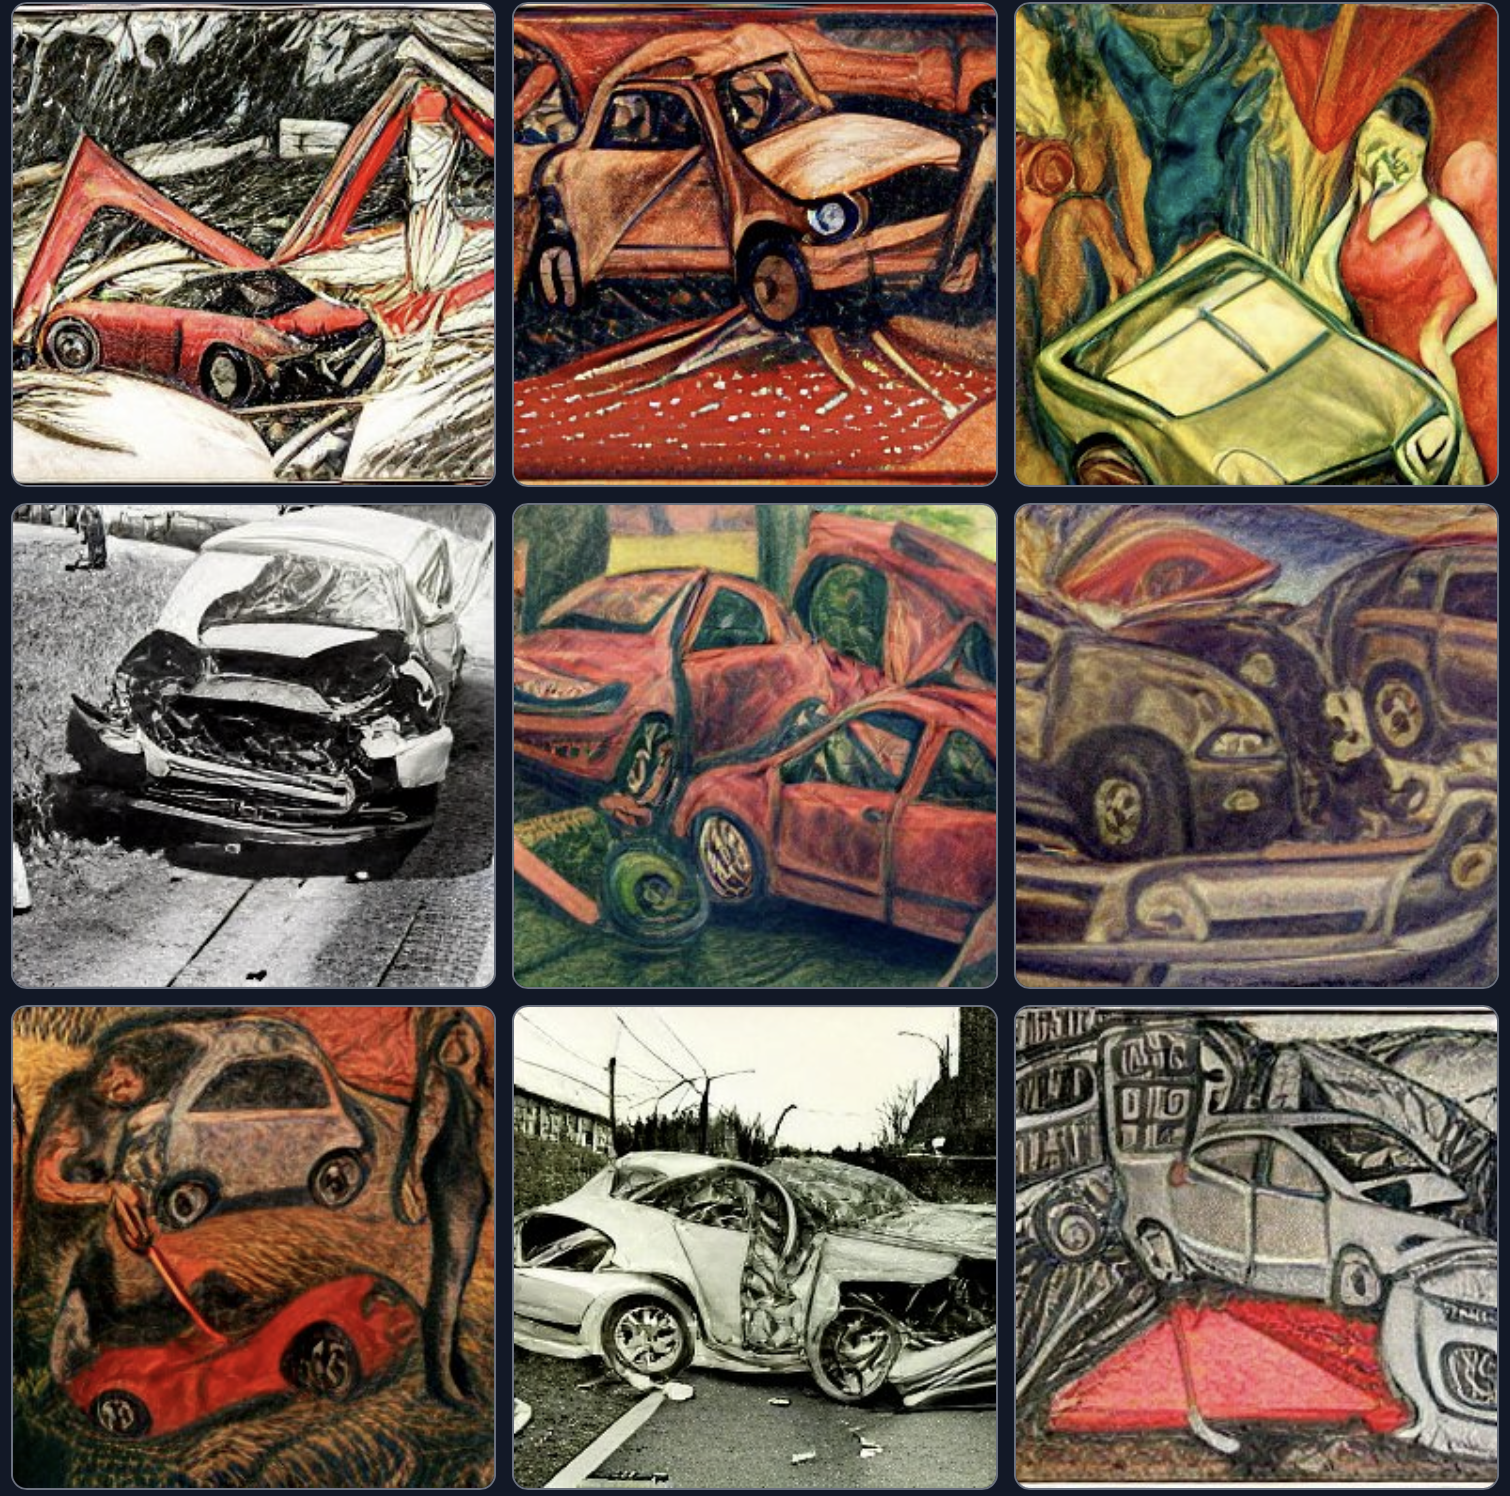
\includegraphics[width=\textwidth]{u1.png}
        \caption{Wynik dla frazy: „two cars crashed into big red triangle, style of witkacy” \cite{6}.\\}
        \label{u1}
     \end{subfigure}
     \hfill
     \begin{subfigure}[H]{0.40\textwidth}
         \centering
         \includegraphics[width=\textwidth]{u2.png}
    \caption{Wynik dla frazy: „two cars crashed into big red triangle, style of stanislaw wyspianski” \cite{6}.\\}
    \label{u2}
     \end{subfigure}
     \centering
     \begin{subfigure}[H]{0.40\textwidth}
        \centering
        \includegraphics[width=\textwidth]{u3.png}
        \caption{Wynik dla frazy: „two cars crashed into big red triangle, style of beksinski” \cite{6}.}
        \label{u3}
     \end{subfigure}
     \hfill
     \begin{subfigure}[H]{0.40\textwidth}
         \centering
         \includegraphics[width=\textwidth]{u4.png}
    \caption{Wynik dla frazy: „two cars crashed into big red triangle, style of jan matejko” \cite{6}.}
    \label{u4}
    \end{subfigure}
\end{figure}

Google oraz DeepMind również zaprezentowały swoje systemy, odpowiednio o nazwach „Imagen” oraz „Flamingo”  \cite{7,8}. Działanie jest bardzo podobne, a rezultaty ciężkie do ocenienia przez zwykłego człowieka niebędącego ekspertem – twierdzą, że jeden model może sprawować się lepiej przy generowaniu np. fotorealistycznych odbić światła, a drugi w grafikach o ujęciu bardziej artystycznym. Jednak na pewno jest to duży krok w sposobie tworzenia grafiki w najbliższej przyszłości – narzędzia zbudowane na podstawie tych modeli mogą znacznie przyśpieszyć procesy kreatywne lub np. całkowicie wyeliminować konieczność odbywania sesji fotograficznych na serwisy oferujące usługi stockowe.

Kolejnym dużym krokiem w przyśpieszeniu tworzenia narzędzi do procesów kreatywnych może być zaprezentowany również przez zespół DeepMind model „Gato” \cite{9}. Jak twierdzą, jest on dopiero w początkowej fazie rozwoju, ale stawia naprawdę solidne fundamenty pod stworzenie systemu odpowiedzialnego za tzw. General AI. Aktualna wersja „Gato” pozwala na rozwiązywanie ponad 600 różnych, niekoniecznie podobnych do siebie problemów, takich jak np. sterowanie ramionami robota, granie w gry wideo, odpowiadanie na pytania z zachowaniem semantyki i gramatyki czy opisywanie, co znajduje się na przedstawionym obrazku. Co ważne, w ponad 75\% tych zadań model dorównuje poziomowi przeciętnego człowieka, a w niektórych nawet znacznie go przewyższa.

Innym, dość popularnym systemem jest „DeepDream” stworzony przez Google w 2015 roku. Program wykorzystuje sieci neuronowe nauczone do wykrywania obrazów. Po modyfikacjach jest w stanie tworzyć obrazy w pewnym stopniu podobne do tych, które ludzkie oko odnotowuje na codzień, jednak przekształcone tak, aby imitowały zjawisko pareidolii czy wywoływały psychodeliczne wrażenia \cite{10}. Jako że rozwiązanie zostało zaproponowane już kilka lat temu, na ten moment powstało wiele aplikacji wykorzystujących przedstawioną architekturę. W 2022 roku grupa badawcza koordynowana przez Uniwersytet w Trydencie zmierzyła kreatywność uczestników po ekspozycji na halucynacyjne filmy generowane przez algorytm „DeepDream”. Po ekspozycji psychodelicznej badane osoby wykazywały się większą kreatywnością. Prawdopodobnie z powodu reorganizacji dynamiki poznawczej, która ułatwia eksplorację nietypowych strategii decyzyjnych i hamuje automatyczne wybory dokonywane przez ludzki mózg, ich automatyczny proces decyzyjny został osłabiony.

Oprócz generowania sztuki strice, te same modele po modyfikacji można zastosować do innych celów w procesach kreatywnych, takich jak np. naprawianie starych fotografii, zwiększanie rozdzielczości zdjęć, automatyczne tworzenie animacji itd. Dodatkowo popularnym, lecz kontrowersyjnym ostatnio tematem, stało się stosowanie NFT (ang. non-fungible token), co również otwiera nowe perspektywy na rynku sztuki cyfrowej.

NFT to unikatowa, cyfrowa jednostka danych oparta na architekturze blockchain, którą użytkownicy protokołu mogą między sobą handlować, reprezentująca szeroką gamę przedmiotów materialnych i niematerialnych, takich jak kolekcjonerskie karty sportowe, wirtualne nieruchomości lub wirtualne dzieła sztuki. Wraz z początkiem 2021 roku artyści, celebryci i sportowcy zaczęli wydawać swoje prace połączone z ich wirtualnymi odpowiednikami NFT. Kupujący dostrzegają w nich wyjątkowy produkt o wartości kolekcjonerskiej, który wraz z upływem lat mógłby zyskać na wartości. Posiadanie danego tokena nie uprawnia nas do praw autorskich obiektu, który reprezentuje; do tego potrzebna jest odpowiednia umowa prawna. Artysta może sprzedać token NFT reprezentujący swoje dzieło, ale nie przekazać kupującemu związanych ze zmianą własności praw. W tym sensie tokeny NFT są odrębne od prawa autorskiego. Kontrowersje dotyczące NFT podnoszą zarzut wysokiego zużycia energii związanego z transakcjami blockchain, co w konsekwencji powoduje wysokie emisje gazów cieplarnianych. Głównym czynnikiem za to odpowiedzialnym jest system Proof of Work wymagany do regulowania i weryfikacji transakcji blockchain w sieciach takich jak Ethereum, które zużywają duże ilości energii elektrycznej \cite{62}. Ponadto, krytycy NFT porównują je do piramid finansowych i baniek spekulacyjnych.

Systemem, któremu poświęcona zostanie dalsza część tej pracy, jest Neuronowy Transfer Stylu (ang. Neural Style Transfer - NST), czyli zastosowanie niektórych z wymienionych wcześniej architektur w celu odwzorowania stylu danego artysty, stosując dowolne zdjęcia na wejściu, a oczekując w zamian grafiki zawierającej ten sam kontekst (to, co obraz wejściowy przedstawiał), lecz kolorystyką i ogólnym klimatem powinien sprawiać wrażenie, jakby było to kolejne dzieło konkretnego artysty.

\begin{figure}[H]
    \centering
    \includegraphics[width=\textwidth]{u5.png}
    \caption{Przykład algorytmu NST przenoszącego styl chińskiego obrazu na dane zdjęcie. Obraz stylu nosi nazwę „Dwelling in the Fuchun Mountains” i jest autorstwa Gongwang Huang \cite{22}.}
    \label{fig:2}
\end{figure}
\newpage

\section{Transfer stylu artystycznego}

\subsection{Wstęp oraz pierwsze publikacje}

\indent

Transfer stylu artystycznego (ang. Artistic Style Transfer) jest możliwy na przekroju wszystkich szerokopojętych mediów, jednak zakres tej pracy skupia się wokół zastosowania w kontekście obrazów. Już w latach dziewięćdziesiątych naukowcy zaczęli interesować się możliwościami komputerów w zakresie przekształcania obrazów w syntetyczne dzieła sztuki, jednak większość z proponowanych przez nich algorytmów stylizacji była zaprojektowana dla konkretnych stylów artystycznych i nie mogła być łatwo rozszerzona na inne style. Wśród społeczności badaczy pracującej nad wizją komputerową transfer stylu jest zwykle badany jako uogólniony problem syntezy tekstury, który polega na wyodrębnieniu i przeniesieniu tekstury ze źródła do celu \cite{22}. Przykładem pierwszych publikacji w tym temacie może być Hertzmann et al., którzy w 2001 roku proponują framework przeznaczony do wykonywania uogólnionego transferu stylu poprzez uczenie analogicznych transformacji na podstawie dostarczonych przykładowych par obrazów niestylizowanych i stylizowanych. Jednak dzielonym ograniczeniem tych metod jest to, że wykorzystują one jedynie niskopoziomowe cechy obrazu i często nie są w stanie skutecznie uchwycić struktur obrazu \cite{23}.

Na przestrzeni późnych lat dziewięćdziesiątych i wczesnych dwutysięcznych powstawało jeszcze kilka innych algorytmów pozwalających na zmianę tekstury stylu obrazu, jednak wszystkie z nich zazwyczaj były mało elastyczne; limitowały je ograniczenia w różnorodności stylów i efektywnej ekstrakcji struktury obrazu \cite{25,26,27,28}. Powyższe problemy poniekąd zostały rozwiązane przez wprowadzenie algorytmów wykorzystujących sieci neuronowe.
\begin{figure}[H]
    \centering
    \includegraphics[width=\textwidth]{u6.png}
    \caption{Analogia obrazu – zadaniem jest obliczenie nowego „analogicznego” obrazu B', który odnosi się do B w „taki sam sposób” jak A' odnosi się do A. A, A' i B są wejściami do naszego algorytmu, a B' jest wyjściem \cite{23}.}
    \label{fig:3}
\end{figure}

\subsection{Wykorzystanie sieci neuronowych}

\indent

Neuronowy Transfer Stylu (ang. Neural Style Transfer, NST) to zbiór algorytmów wykorzystujący sieci neuronowe do rozwiązania zagadnienia przeniesienia stylu obrazu na inny.

Podstawowa idea tego podejścia polega najpierw na wyodrębnieniu informacji o stylu i zawartości (treści) obu obrazów podawanych na wejściu, a następnie iteracyjnej rekombinacji wyniku tak długo, aż rekonstrukcja obrazu docelowego będzie pasowała do wyodrębnionej wcześniej reprezentacji stylu. Wspólnym ograniczeniem tego typów algorytmów jest to, że ze względu na iteracyjną procedurę optymalizacji obrazu są one kosztowne obliczeniowo.

\subsubsection{Geneza}

\indent

Przed przedstawieniem dokładnego działania takiego algorytmu, należy najpierw wspomnieć o konwolucyjnej sieci neuronowej VGG-19. W roku 2012 zaproponowano rozwiązanie, które przez wielu opisane jest przełomowym – do rozwiązania konkursu ImageNet polegającego na stworzeniu jak najlepszego algorytmu rozpoznawania obiektów na zdjęciu zgłoszono sieć AlexNet korzystającą z konwolucji \cite{32}. Od tego czasu sieci konwolucyjne stały się standardem w kontekście pracy z wizją komputerową.

W 2013 powstała publikacja prezentująca w jaki sposób sieć neuronowa, a raczej jej kolejne warstwy, postrzegają prezentowany obraz \cite{33}. Autorzy zbadali, dlaczego konwolucyjne sieci neuronowe osiągają tak dobre wyniki i w jaki sposób można by je jeszcze poprawić. Zaproponowali nową technikę wizualizacji, która daje wgląd w funkcje pośrednich warstw cech i działanie klasyfikatora. Przedstawiona została idea głosząca, że w niższych warstwach analizowane są prostsze struktury geometryczne, a wraz z zagłębianiem się w dalsze warstwy – bardziej złożone.
\begin{figure}[H]
    \centering
    \includegraphics[width=\textwidth]{u7.png}
    \caption{Wizualizacja cech pozwala nam zobaczyć, jak GoogLeNet wytrenowany na zbiorze danych ImageNet buduje swoje rozumienie obrazów na przestrzeni wielu warstw \cite{61}.}
    \label{fig:4}
\end{figure}

Rok później, w 2014 roku, zwycięzcą kolejnej edycji konkursu ImageNet została sieć VGG-19 oferująca większą precyzję i głębię w porównaniu do jej poprzedników \cite{34}. Autorzy skupili się na zbadaniu wpływu głębokości sieci konwolucyjnej na jej dokładność w warunkach rozpoznawania obrazów na dużą skalę. Skupiono się na ocenie sieci o rosnącej głębokości przy użyciu architektury z bardzo małymi (3 × 3) filtrami konwolucyjnymi, która pokazała, że znaczącą poprawę w stosunku do konfiguracji poprzedników można osiągnąć poprzez przesunięcie głębokość do 16-19 warstw. Zespół zapewnił sobie pierwsze i drugie miejsce odpowiednio w kategorii lokalizacji i klasyfikacji. Autorzy udostępnili publicznie dwa najlepsze modele ConvNet, aby ułatwić dalsze badania nad wykorzystaniem głębokich reprezentacji wizualnych w widzeniu komputerowym.

Publikacja pod tytułem „Understanding Deep Image Representations by Inverting Them” przedstawiła sposób na odtworzenie obrazu, bazując na jego reprezentacji w sieci neuronowej \cite{35}. Praca ta była fundamentem do powstania systemu „DeepDream”, o którym mowa była już w poprzednich rozdziałach \cite{10}.
\begin{figure}[H]
    \centering
    \includegraphics[width=\textwidth]{u8.png}
    \caption{Rekonstrukcja obrazu w każdej z warstw CNN \cite{35}.}
    \label{fig:5}
\end{figure}

Wykorzystując właściwości VGG-19, w 2015 roku Gatys et al. zaprezentowali publikację dotyczącą syntezy tekstury zdjęć, a konkretniej – obliczeń statystki macierzy Grama z wykorzystaniem niskowarstwowych cech sieci \cite{24}. W modelu tekstury są reprezentowane przez korelacje pomiędzy mapami cech w kilku warstwach sieci. Pokazano, że w poszczególnych warstwach reprezentacje tekstur coraz lepiej oddają statystyczne właściwości naturalnych obrazów, jednocześnie coraz bardziej uwypuklając informacje o obiektach.

\subsubsection{Pierwszy algorytm neuronowego transferu stylu}

\indent

Wszystkie publikacje przedstawione powyżej zostały niejako połączone, tworząc nowy koncept – neuronowy transfer stylu. Pierwszy algorytm został przedstawiony również przez zespół Gatysa et al. w 2015 roku \cite{19}. Wykorzystuje on pre-trenowaną sieć VGG-19 stosowaną do rozpoznawania obrazów. Poprzez rekonstrukcję reprezentacji z warstw sieci VGG-19, sieć neuronowa jest w stanie wyodrębnić treść obrazu z dowolnego zdjęcia oraz pewną informację o stylu z podanego dzieła sztuki. Mając tę informację, obraz wejściowy jest iteracyjne nadbudowywany nowym stylem, stosując do tego celu dopasowanie oparte na sumarycznej statystyce macierzy Grama obliczane z wykorzystaniem oryginalnego stylu \cite{24}. Szczegóły ich algorytmu są następujące.

Biorąc pod uwagę obraz treści (ang. content image) $I_c$ i obraz stylu (ang. style image) $I_s$, algorytm próbuje iteracyjnie szukać obrazu stylizowanego $I$, który minimalizuje następującą funkcję celu:
\begin{align*}
    I^*=\text{argmin}\ L_{\text{total}}\left(I_c,I_s,I\right) = \text{argmin}\ \alpha L_{C}\left(I_c,I\right)+\beta L_s\left(I_s,I\right),
\end{align*}
gdzie $L_c$ porównuje reprezentację treści danego obrazu z reprezentacją stylizowanego obrazu, a $L_s$ porównuje reprezentację stylu opartą na metodzie Grama uzyskaną ze stylizowanego obrazu z reprezentacją stylizowanego obrazu, natomiast $\alpha$ i $\beta$ są używane do zrównoważenia składowej treści i składowej stylu w stylizowanym wyniku.

Strata zawartości (ang. content loss) $L_c$ jest określona przez kwadrat odległości euklidesowej między reprezentacjami cech $F^l$ obrazu treści $I_c$ w warstwie $l$, a reprezentacją obrazu stylizowanego $I$, który na początku jest inicjalizowany białym szumem:
\begin{align*}
    L_c = \Sigma_{l\in \{l_c\}}\left|\left|F^l\left(I_c\right)-F^l(I)\right|\right|^2,
\end{align*}
gdzie $\{l_c\}$ oznacza zbiór warstw sieci VGG służących do obliczenia straty zawartości.

Dla straty stylu $L_s$ wykorzystano technikę modelowania tekstury wizualnej opartą na Gramie do modelowania stylu \cite{24}. Dlatego strata stylu jest definiowana przez kwadrat odległości euklidesowej pomiędzy opartymi na Gramie reprezentacjami stylu $I_s$ i $I$:
\begin{align*}
    L_s = \Sigma_{l\in \{l_s\}}\left|\left|G\left(F^l\left(I_s\right)'\right)-G\left(F^l(I)'\right)\right|\right|^2,
\end{align*}
gdzie $G$ to wspomniana wcześniej macierz Grama kodująca statystyki zbioru filtrów. $\{l_s\}$ reprezentuje zbiór warstw VGG służących do obliczania strat stylu.

Wybór warstw zawartości i stylu jest ważnym czynnikiem w procesie przenoszenia stylów. Inne pozycje i liczba warstw mogą skutkować bardzo różnymi doświadczeniami wizualnymi. Biorąc pod uwagę wstępnie wytrenowaną sieć VGG-19, Gatys et al. wybrali zbiory $\{l_s\}$ i $\{l_c\}$, wybierając odpowiednio warstwy; dla $\{l_s\}$ = $\{\text{conv}1_1, \text{conv}2_1, \text{conv}3_1, \text{conv}4_1, \text{conv}5_1\}$ oraz dla $\{l_c\} = \{\text{conv}4_2\}$.
\begin{figure}[H]
    \centering
    \includegraphics[scale=0.65]{u9.png}
    \caption{Ilustracja architektury sieciowej modelu VGG-19 \cite{31}.}
    \label{fig:6}
\end{figure}

Dla $\{l_s\}$ idea łączenia wielu warstw (aż do najwyższych) jest krytyczna dla sukcesu algorytmu Gatysa. Dopasowanie wielowymiarowych reprezentacji stylów prowadzi do gładszej i bardziej ciągłej stylizacji, co daje najbardziej atrakcyjne wizualnie rezultaty. Dla warstwy treści $\{l_c\}$ dopasowanie reprezentacji zawartości na niższych warstwach zachowuje niepożądane drobne struktury (np. krawędzie i mapę kolorów) oryginalnego obrazu podczas stylizacji. Dla kontrastu, poprzez dopasowanie zawartości na wyższej warstwie sieci, drobne struktury mogą być zmienione tak, aby zgadzały się z pożądanym stylem przy jednoczesnym zachowaniu informacji o treści obrazu. Również wykorzystanie sieci opartych na VGG do przenoszenia stylów nie jest jedyną możliwością. Podobną wydajność można uzyskać wybierając inne wstępnie wytrenowane sieci klasyfikacyjne, np. ResNet \cite{30}.

W równaniu (1) zarówno $L_c$, jak i $L_s$, są różniczkowalne. Tak więc przy losowym szumie jako początkowym $I$, równanie (1) może być minimalizowane poprzez zastosowanie metody gradientu prostego (ang. gradient descent) w przestrzeni obrazu z propagacją wsteczną.

Algorytm Gatysa et al. nie potrzebuje danych prawdy podstawowej (ang. ground truth) do treningu, a także nie ma wyraźnych ograniczeń co do typu obrazów stylizacji, co rozwiązuje ograniczenia poprzednich algorytmów. Jednak algorytm ten nie radzi sobie dobrze z zachowaniem spójności drobnych struktur i szczegółów. Wynika to z istoty działania CNN, w którym cechy (ang. features) naturalnie tracą pewne niskopoziomowe informacje. Ponadto generalnie zawodzi w przypadku syntezy fotorealistycznej ze względu na ograniczenia reprezentacji stylu opartej na Gramie. Dodatkowo nie uwzględnia on odmian pociągnięć pędzla oraz semantyki i informacji o głębi zawartych w obrazie treści, które są ważnymi czynnikami w ocenie jakości wizualnej.

Na bazie tego podejścia powstało parę innych algorytmów próbujących rozwiązać przedstawione wyżej problemy. Li i Wand zaproponowali technikę kodowania stylu bez użycia macierzy Grama \cite{38}. Głównym wkładem algorytmu jest teoretyczne wykazanie, że proces dopasowania macierzy Grama w NST jest równoważny minimalizacji MMD (ang. Maximum Mean Discrepancy) z jądrem wielomianowym drugiego rzędu, proponując w ten sposób aktualną interpretację NST i czyniąc zasadę NST jaśniejszą.

Jednym z ograniczeń algorytmu opartego na metodzie Grama jest jego niestabilność podczas optymalizacji. Ponadto wymaga on ręcznego dostrajania parametrów, co jest bardzo uciążliwe. Risser et al. stwierdzają, że aktywacje cech o całkiem różnych średnich i wariancjach mogą nadal mieć tę samą macierz Grama, co jest główną przyczyną niestabilności \cite{36}. Zainspirowani tą obserwacją, Risser et al. wprowadzili dodatkową stratę histogramową, która kieruje optymalizacją w celu dopasowania całego histogramu aktywacji cech. Przedstawili również wstępne rozwiązanie automatycznego dostrajania parametrów polegające na jawnym zapobieganiu gradientom o skrajnych wartościach poprzez normalizację gradientu ekstremalnego. Dzięki dodatkowemu dopasowaniu histogramu aktywacji cech, algorytm osiąga bardziej stabilne przeniesienie stylu przy mniejszej liczbie iteracji i wysiłków związanych z dostrajaniem parametrów, jednak kosztem tego jest wysoka złożoność obliczeniowa. Ponadto nadal istnieją wspomniane wcześniej słabości algorytmu Gatysa et al., np. brak uwzględnienia głębi i spójności szczegółów.

Wszystkie wymienione wcześniej metody porównują jedynie treść i stylizowane obrazy w przestrzeni cech CNN, aby uczynić stylizowany obraz semantycznie podobnym do obrazu treści. Ponieważ jednak cechy CNN nieuchronnie tracą pewne niskopoziomowe informacje zawarte w obrazie, w wynikach stylizacji pojawiają się zwykle pewne nieatrakcyjne, zniekształcone struktury i nieregularne elementy graficzne. Aby zachować spójność drobnych struktur podczas stylizacji, Li et al. zaproponowali wprowadzenie dodatkowych ograniczeń dla cech niskopoziomowych w przestrzeni pikseli \cite{37}. Wprowadzili oni dodatkową stratę Laplace’a, która jest zdefiniowana jako kwadratowa odległość euklidesowa pomiędzy odpowiedziami filtru Laplace’a obrazu treści i stylizowanego wyniku. Filtr Laplace’a oblicza pochodne drugiego rzędu pikseli w obrazie i jest szeroko stosowany przy problemie wykrywania krawędzi.

Algorytm Li et al. ma dobre wyniki w zakresie wstępnej obsługi drobnych struktur i szczegółów podczas stylizacji, jednak nadal brakuje w nim rozważań na temat semantyki, głębi, różnic w pociągnięciach pędzla, etc.

Kolejna metoda rozpatruje NST na poziomie lokalnym, tj. operuje na łatach (ang. patches) w celu dopasowania stylu. Li i Wand jako pierwsi zaproponowali algorytm NST wykorzystujący tę cechę. Stwierdzili, że parametryczna metoda NST ze statystyką sumaryczną ujmuje jedynie korelacje cech per-pikselowych i nie ogranicza układu przestrzennego, co prowadzi do mniej wiarygodnego wizualnie wyniku dla fotorealistycznych stylów \cite{38}. Ich rozwiązaniem jest modelowanie stylu w sposób nieparametryczny i wprowadzenie nowej funkcji straty stylu, która zawiera priorytety MRF oparte na łatach:
\begin{align*}
    L_s = \Sigma_{l\in \{l_s\}}\sum_{i=1}^{m}\left|\left|\Psi_i\left(F^l(I)\right)-\Psi_{NN(i)}\left(F^l\left(I_s\right)\right)\right|\right|^2,
\end{align*}
gdzie $\Psi(F^l(I))$ to zbiór wszystkich lokalnych łat z mapy cech $(F^l(I)$. $\Psi_i$ oznacza i-tą łatę lokalną, a $\Psi_{NN(i)}$ jest najbardziej podobną łatą stylistyczną z i-tą łatą lokalną w obrazie stylizowanym $I$. Najlepsze dopasowanie $\Psi_{NN(i)}$ uzyskuje się przez obliczenie znormalizowanej korelacji krzyżowej nad wszystkimi łatami stylu w obrazie stylizowanym $I_s$. $m $ to całkowita liczba łat lokalnych.

Ponieważ ich algorytm dopasowuje styl na poziomie łat, struktura i układ są zachowywane znacznie lepiej. Zaletą algorytmu Li i Wand jest również to, że sprawdza się on szczególnie dobrze dla fotorealistycznych stylów, a dokładniej – gdy zdjęcie zawartości i styl są podobne pod względem kształtu i perspektywy, jednak generalnie zawodzi, gdy zdjęcia treści i stylu mają silne różnice w perspektywie i strukturze, ponieważ łaty obrazu nie mogą być poprawnie dopasowane. Jest również ograniczony w zachowywaniu ostrych szczegółów i informacji o głębi.

\subsection{NST w czasie rzeczywistym – modelowanie stylów}

\indent

Najbardziej istotnym ograniczeniem algorytmów przedstawionych w poprzednim rozdziale jest kwestia wydajności. W tym rozdziale przedstawione zostaną metody rozwiązujące problem szybkości i kosztów obliczeniowych, wykorzystując optymalizację opartą na modelowaniu (ang. Model-Optimisation-Based) do rekonstrukcji wystylizowanego wyniku, tzn. sieć typu feed-forward jest optymalizowana na dużym zbiorze obrazów $I_c$ dla jednego lub więcej obrazów stylu $I_s$:
\begin{align*}
    \theta^*=\text{argmin}\ L_{\text{total}}\left(I_c,I_s,g_{\theta^*}\left(I_c\right)\right),\ I^*=g_{\theta^*}\left(I_c\right).
\end{align*}
Metody te można skategoryzować ze względu na liczbę stylów, które pojedynczy model $g$ jest w stanie wyprodukować:

\begin{itemize}
    \item Per-Style-Per-Model (PSPM),
    \item Multiple-Style-Per-Model (MSPM),
    \item Arbitrary-Style-Per-Model (ASPM).
\end{itemize}

\subsubsection{Per-Style-Per-Model (PSPM)}

\indent

Pierwsze dwa algorytmy z tej kategorii zostały zaproponowane odpowiednio przez Johnsona et al. \cite{39} oraz Ulyanova et al. \cite{40}. Te dwie metody mają podobną ideę, która polega na wstępnym wytrenowaniu sieci feed-forward specyficznej dla stylu i następnie wytworzeniu stylizowanego wyniku za pomocą jednego przejścia w przód podczas fazy testowania. Różnią się jedynie architekturą sieci, w przypadku której projekt Johnsona et al. wykorzystuje bloki szczątkowe (ang. residual blocks) oraz cząstkowo kroczące konwolucje (ang. fractionally-strided convolutions), a Uljanow et al. wykorzystują architekturę wieloskalową jako sieć generującą. Funkcja celu jest podobna do algorytmu Gatysa. Algorytmy Johnsona oraz Ulyanova są w stanie osiągnąć transfer stylu w czasie rzeczywistym, jednak ich konstrukcja w zasadzie imituje algorytm Gatysa, co sprawia, że cierpią one na te same wspomniane wcześniej problemy (np. brak uwzględnienia w spójności szczegółów i informacji o głębi).

Niedługo później Ulyanov et al. stwierdzili, że samo zastosowanie normalizacji do każdego pojedynczego obrazu zamiast do batcha obrazów (ang. batch normalization, BN) prowadzi do znacznej poprawy jakości stylizacji \cite{41}. Ta normalizacja pojedynczego obrazu jest nazywana normalizacją instancji (ang. instance normalisation, IN), która jest równoważna normalizacji batcha, gdy rozmiar batcha jest ustawiony na 1. Wykazano, że sieć przenoszenia stylu z IN działa szybciej niż BN, a także osiąga wizualnie lepsze wyniki. Jedną z interpretacji jest to, że IN jest pewnego rodzaju formą normalizacji stylu i może bezpośrednio normalizować styl każdego obrazu zawartości do pożądanego. Dzięki temu, że reszta sieci zajmuje się utratą treści (ang. content loss), cel jest łatwiejszy do nauczenia.

Kolejna praca Li i Wand jest inspirowana algorytmem NST przedstawionym w ich poprzedniej pracy, która została omówiona w poprzednich podrozdziałach. Rozwiązują oni problem wydajności poprzez trenowanie markowskiej sieci feed-forward z wykorzystaniem architektury GAN \cite{42}. Podobnie jak ich ostatni algorytm, ta metoda operuje na łatach. Wykazano, że ich metoda przewyższa algorytmy Johnsona oraz Ulyanova w zachowaniu spójnych tekstur w złożonych obrazach właśnie dzięki konstrukcji opartej na łatach. Jednakże ich algorytm ma mniej satysfakcjonującą wydajność w przypadku stylów innych niż tekstury (np. obrazy twarzy), ponieważ nie uwzględnia semantyki. Inne słabości algorytmu to brak uwzględnienia informacji o głębi i zmienności pociągnięć pędzla, które są ważnymi czynnikami wizualnymi.

\subsubsection{Multiple-Style-Per-Model (MSPM)}

Chociaż powyższe metody PSPM mogą tworzyć stylizowane obrazy o dwa rzędy wielkości szybciej niż poprzednie metody, to dla każdego obrazu stylizowanego trzeba wytrenować oddzielne sieci generatywne, co jest dość czasochłonne i mało elastyczne. Jednak wiele obrazów (np. obrazy impresjonistyczne) ma podobne pociągnięcia farby i różni się jedynie paletą kolorów. Intuicyjnie, trenowanie osobnej sieci dla każdego z nich jest zbędne. Proponuje się zatem MSPM, który zwiększa elastyczność PSPM poprzez dalsze włączenie wielu stylów do jednego modelu. Istnieją dwie drogi rozwiązania tego problemu: 1) powiązanie tylko niewielkiej liczby parametrów w sieci z każdym stylem i 2) dalsze wykorzystywanie tylko jednej sieci jak PSPM, ale łączącej zarówno styl, jak i treść jako dane wejściowe.

\begin{enumerate}
    \item \textbf{Powiązanie z każdym stylem tylko niewielkiej liczby parametrów}
\end{enumerate}   

Wczesna praca Dumoulin et al. jest zbudowana na podstawie zaproponowanej wcześniej metody wykorzystującej IN w algorytmie PSPM \cite{43}. W zaskakujący sposób badacze zauważyli, że używając tych samych parametrów konwolucyjnych, a jedynie skalując i przesuwając parametry w warstwach IN, możliwe jest modelowanie różnych stylów. W związku z tym zaproponowano algorytm trenowania warunkowej wielostylowej sieci transferowej oparty na warunkowej normalizacji instancji (ang. conditional instance normalisation, CIN), która jest zdefiniowana jako:
\begin{align*}
    \text{CIN}\left(F\left(I_c\right),s\right)= \gamma^s\left( \frac{F\left(I_c\right)-\mu\left(F\left(I_c\right)\right)}{\sigma\left(F\left(I_c\right)\right)}\right)+\beta^s,
\end{align*}
gdzie $F$ jest wejściową aktywacją cechy, a $s$ jest indeksem pożądanego stylu ze zbioru stylów. Jak wynika z równania, warunkowanie dla każdego stylu $I_s$ odbywa się poprzez skalowanie i zmianę parametrów $\gamma^s$ i $\beta^s$ po normalizacji aktywacji cechy $F(I_c)$, czyli każdy styl $I_s$ można uzyskać poprzez dostrojenie parametrów transformacji afinicznej. Algorytm Dumoulin et al. może być również rozszerzony do łączenia wielu stylów w pojedynczy wynik stylizacji poprzez łączenie parametrów afinicznych różnych stylów.

Inny algorytm zaproponowali Chen et al. \cite{44}. Ich pomysł polega na wyraźnym rozdzieleniu stylu i treści, tj. użyciu oddzielnych komponentów sieci do uczenia się odpowiednich informacji o treści i stylu. Dokładniej używają oni filtrów konwolucyjnych średniego poziomu (zwanych warstwą „StyleBank”) do indywidualnego uczenia się różnych stylów. Każdy styl jest związany z zestawem parametrów w warstwie „StyleBank”. Pozostałe elementy sieci są wykorzystywane do uczenia się informacji o treści, która jest wspólna dla różnych stylów. Algorytm wspiera również elastyczny trening przyrostowy (ang. flexible incremental training), który polega na ustaleniu komponentów treści w sieci i trenowaniu tylko warstwy „StyleBank” dla nowego stylu.

Podsumowując, zarówno algorytmy Dumoulin et al., jak i Chen et al., mają zalety w postaci niewielkiego wysiłku potrzebnego do nauczenia się nowego stylu oraz elastycznej kontroli nad fuzją stylów. Nie rozwiązują one jednak typowych ograniczeń algorytmów NST, np. braku szczegółów, semantyki, głębi i wariacji pociągnięć pędzla.
\begin{enumerate}
    \setcounter{enumi}{1}
    \item \textbf{Łączenie zarówno stylu, jak i treści jako danych wejściowych}
\end{enumerate}

Jedną z wad pierwszej kategorii jest to, że rozmiar modelu generalnie staje się większy wraz ze wzrostem liczby uczonych stylów. Druga ścieżka MSPM rozwiązuje to ograniczenie poprzez pełne wykorzystanie możliwości jednej sieci i połączenie zarówno treści, jak i stylu w sieci do identyfikacji stylu. Różne algorytmy MSPM różnią się sposobem włączenia stylu do sieci.

Li et al., biorąc pod uwagę N docelowych stylów, zaprojektowali jednostkę selekcji dla wyboru stylu, która jest N-wymiarowym wektorem typu one-hot. Każdy bit w jednostce wyboru reprezentuje określony styl $I_s$ w zbiorze stylów docelowych \cite{45}. Dla każdego bitu w jednostce selekcji, Li et al. najpierw próbkują odpowiednią mapę szumu $f(I_s)$ z jednolitego rozkładu, a następnie wprowadzają $f(I_s)$ do podsieci stylów, aby uzyskać odpowiednie cechy zakodowane w stylu $F(f(I_s))$. Wprowadzając konkatenację cech zakodowanych stylem $F(f(I_s))$ i cech zakodowanych treścią $Enc(I_c)$ do części dekodera $Dec$ sieci transferu stylu, można uzyskać pożądany wynik stylizacji:
    \begin{align*}
        I = \text{Dec}\left(F\left(f\left(I_s\right)\right) \oplus \text{Enc}\left(I_c\right)\right).
    \end{align*}
Inna praca Zhanga i Dana najpierw przekazuje każdy obraz stylizacji w zbiorze stylizacji przez wstępnie wytrenowaną sieć VGG, a następnie uzyskuje wieloskalowe aktywacje cech $F(I_s)$ w różnych warstwach VGG \cite{46}.

Następnie wieloskalowe $F(I_s)$ są łączone z wieloskalowymi zakodowanymi cechami $F(I_s)$ z różnych warstw w enkoderze poprzez zaproponowane przez nich warstwy inspiracji. Warstwy inspiracji są zaprojektowane tak, aby przekształcić $F(I_s)$ i dopasować go do pożądanego wymiaru, a także posiadają trenowalną macierz wag, by dostroić mapy cech w celu zminimalizowania funkcji celu.

Drugi typ MSPM rozwiązuje ograniczenie wynikające ze zwiększonego rozmiaru modelu w pierwszym typie MSPM. Kosztem tego skalowalność stylu w drugim typie MSPM jest znacznie mniejsza, ponieważ tylko jedna sieć jest używana dla wielu stylów. Ponadto, pewne wspomniane wcześniej ograniczenia pierwszego typu MSPM nadal istnieją, tzn. drugi typ algorytmów MSPM jest nadal ograniczony w zachowaniu spójności drobnych struktur, a także informacji o głębi.

\subsubsection{Arbitrary-Style-Per-Model (ASPM)}

\indent

Trzecia kategoria ma na celu stworzenie jednego modelu dla wszystkich, tzn. jednego modelu, który można wytrenować, aby przenieść dowolne style artystyczne. Istnieją również dwa rodzaje ASPM – jeden zbudowany na bazie nieparametrycznego modelowania tekstury, a drugi na bazie parametrycznego modelowania tekstury ze statystyką sumaryczną.

\noindent\textbf{Nieparametryczny ASPM}

Pierwszy algorytm ASPM zaproponowali Chen i Schmidt \cite{47}. W pierwszej kolejności wyodrębnili oni zestaw łat aktywacji z aktywacji cech treści i stylu obliczonych we wstępnie wytrenowanej sieci VGG. Następnie dopasowali każdą łatę treści do najbardziej podobnej łaty stylu i zamienili je (nazywając tę czynność „Style Swap”). Stylizowany wynik można uzyskać poprzez rekonstrukcję wynikowej mapy aktywacji po „Style Swap” za pomocą technik zaprezentowanych w poprzednich rozdziałach. Algorytm Chena i Schmidta jest bardziej elastyczny niż poprzednie podejścia ze względu na jego charakterystykę – jeden model dla wielu stylów (ang. one-model-for-all-style). Jednak stylizowane wyniki są mniej atrakcyjne, ponieważ łaty treści są zwykle zamieniane z łatami stylu, które nie są reprezentatywne dla pożądanego stylu. W rezultacie treść jest dobrze zachowana, podczas gdy styl nie jest na ogół dobrze odzwierciedlony.
    
\noindent\textbf{Parametryczny ASPM ze statystyką sumaryczną}

Biorąc pod uwagę pracę Dumoulina przedstawioną w poprzednim rozdziale, najprostszym podejściem do arbitralnego przenoszenia stylów jest wytrenowanie oddzielnej sieci predykcji parametrów P do przewidywania $\gamma^s$ i $\beta^s$ w równaniu CIN (przedstawionym powyżej) za pomocą pewnej liczby stylów treningowych \cite{48}. Biorąc pod uwagę obraz stylu testowego $I_s$, warstwy CIN w sieci transferu stylu pobierają afiniczne parametry $\gamma^s$ i $\beta^s$ z $P(I_s)$ i normalizują wejściowy obraz zawartości do pożądanego stylu.

Inne podobne podejście oparte na tej pracy proponują Huang i Belongie \cite{49}. Zamiast trenować sieć predykcji parametrów, Huang i Belongie proponują modyfikację warunkowej normalizacji instancji (ang. conditional instance normalisation, CIN) na adaptacyjną normalizację instancji (ang. adaptive instance normalisation, AdaIN):

\begin{align*}
    \text{AdaIN}\left(F\left(I_c\right),F\left(I_s\right)\right) = \sigma\left(F\left(I_s\right)\right)\left(\frac{F\left(I_c\right)-\mu\left(F\left(I_c\right)\right)}{\sigma\left(F\left(I_c\right)\right)}\right)+\mu\left(F\left(I_s\right)\right).
\end{align*}

AdaIN przenosi średnią i wariancję statystyk cech pomiędzy aktywacjami cech treści i stylu. Koder w sieci transferu stylu w pracy Huanga i Belongie jest stały i obejmuje kilka pierwszych warstw wstępnie wytrenowanej sieci VGG. Dekoder musi być wytrenowany dużym zestawem obrazów stylu i treści, aby zdekodować wynikowe aktywacje cech po AdaIN do wystylizowanego wyniku:
\begin{align*}
    I = \text{Dec}\left( \text{AdaIN}\left(F\left(I_c\right), F\left(I_s\right)\right)\right).
\end{align*}

Algorytm Huanga i Belongie jest pierwszym algorytmem ASPM, który osiąga stylizację w czasie rzeczywistym. Jednakże jest mocno oparty na danych i ma ograniczone możliwości uogólniania na niewidziane wcześniej style. Ponadto proste dopasowanie średniej i wariancji statystyk cech utrudnia syntezę skomplikowanych wzorców stylów z bogatymi szczegółami i strukturami lokalnymi.

\subsection{Neural Neighbor Style Transfer}

\indent

Zespół Adobe pod kierownictwem Nicka Kolkina w 2022 roku zaproponował zupełnie nowe podejście. Dotychczas dominujące rozwiązania transferu stylu opierały się na oddzielnym zdefiniowaniu straty stylu i straty treści, a następnie znalezieniu obrazu, który kompromisowo minimalizuje oba te czynniki.

Wyzwanie związane z działaniem w tym systemie polega na tym, że sformułowania zaproponowane do tej pory dla straty treści i straty stylu są zasadniczo sprzeczne i generalnie niemożliwe do jednoczesnego doprowadzenia do zera.

W pracy „Less is More, Faithful Style Transfer without Content Loss” autorzy pokazali, że wyraźna strata treści jest zbędna \cite{31}. Zaproponowano algorytm Neural Neighbour Style Transfer (NNST), czyli proste podejście oparte na najbliższych sąsiadach, które pozwala osiągnąć wyższą jakość stylizacji niż wcześniejsze prace bez poświęcania informacji w treści.

\begin{figure}[H]
    \centering
    \includegraphics[width=\textwidth]{u10.png}
    \caption{Architektura zaproponowana przy podejściu NNST \cite{31}.}
    \label{fig:7}
\end{figure}

\subsection{Wyzwania}

\indent

Chociaż obecne algorytmy są już w stanie osiągać dobre wyniki, nadal istnieje kilka wyzwań oraz problemów wymagających zaadresowania.

\subsubsection{Metodologia ewaluacji estetycznej}

\indent

Parametry takie jak czas potrzebny na wygenerowanie obrazu lub zasoby potrzebne do wytrenowania modelu są łatwo mierzalne. Problem pojawia się, gdy wynik chcemy ocenić jakościowo. Ocena estetyczna jest krytycznym zagadnieniem przy NST, a problem ten staje się coraz bardziej krytyczny w miarę dojrzewania tej dziedziny. Badacze potrzebują pewnych wiarygodnych kryteriów do oceny korzyści z proponowanego przez nich podejścia w stosunku do wcześniejszych rozwiązań, a także sposobu na ocenę przydatności jednego konkretnego podejścia do jednego konkretnego scenariusza. Większość prac ocenia proponowane przez siebie podejście za pomocą subiektywnych porównań wizualnych side-by-side lub poprzez pomiary pochodzące z różnych nieustandaryzowanych badań użytkowników.

Na przykład aby ocenić proponowany uniwersalny algorytm przenoszenia stylów, Li et al. przeprowadzili badanie wśród użytkowników, które polegało na poproszeniu uczestników o zagłosowanie na ich ulubione stylizowane wyniki. Nie jest to optymalne rozwiązanie, ponieważ wyniki bardzo się różnią w przypadku różnych obserwatorów.

W innych badaniach zauważono, że biorąc pod uwagę ten sam wystylizowany wynik, różni obserwatorzy z tym samym zawodem i wiekiem nadal mają całkiem różne oceny \cite{22}. Mimo to nie ma obecnie złotego standardu oceny algorytmów NST. To wyzwanie związane z oceną estetyczną pozostanie otwartą kwestią w społeczności NST, której rozwiązanie może wymagać współpracy z profesjonalnymi artystami i wysiłku w zakresie identyfikacji podstawowych zasad estetycznych.

\noindent\textbf{Benchmark dataset}

W dziedzinie NST istnieje jeszcze jedna ważna kwestia związana z oceną estetyczną. Obecnie nie istnieje standardowy zestaw obrazów wzorcowych do oceny algorytmów NST. Różni autorzy zazwyczaj używają własnych obrazów do oceny.

Aby porównać skalowalność stylów różnych metod NST, kluczowe jest poszukiwanie wzorcowego zbioru stylów, który kolektywnie wykazuje szeroki zakres możliwych właściwości wraz ze szczegółowym opisem przyjętych zasad, numerycznymi pomiarami cech obrazów, a także dyskusją ograniczeń. Poszukiwanie wzorcowego zbioru obrazów NST jest dość odrębnym i ważnym kierunkiem badawczym, który daje nie tylko możliwość wykazania przez badaczy poprawy proponowanego przez nich podejścia w stosunku do dotychczasowych rozwiązań, ale również narzędzie do pomiaru przydatności jednego konkretnego algorytmu NST do jednego konkretnego wymagania. Ponadto w związku z pojawieniem się rozszerzeń NST, kolejnym otwartym problemem pozostaje zbadanie specjalistycznego zestawu danych wzorcowych, a także odpowiednich kryteriów oceny tych rozszerzonych prac (np. transfer stylu wideo, transfer stylu audio, transfer stylu stereoskopowego, transfer stylu postaci i transfer stylu mody).

\subsubsection{Interpretacja NST}

\indent

Kolejnym trudnym problemem jest interpretowalność algorytmów NST. Podobnie jak wiele innych zadań związanych z wizją komputerową, proces NST można opisać określeniem „czarna skrzynka” (ang. black box) – w wielu przypadkach nie wiemy, dlaczego model zwrócił dany wynik, co czyni go dość niekontrolowanym.

\noindent\textbf{Wyodrębnienie reprezentacji stylu}

Celem jest nauczenie się interpretowalnych wymiarowo reprezentacji, w których pewne zmiany w jednym lub kilku specyficznych wymiarach odpowiadają zmianom dokładnie w jednym czynniku zmienności, będąc jednocześnie niezmiennikami innych czynników. W transferze stylu, gdyby można było nauczyć się reprezentacji, w której czynniki zmienności (np. kolor, kształt, wielkość kreski, orientacja kreski i skład kreski) są precyzyjnie rozłączone, czynniki te mogłyby być następnie dowolnie kontrolowane podczas stylizacji. Na przykład można by zmienić orientację kreski w stylizowanym obrazie, zmieniając po prostu wymiar odpowiadający w wyuczonym rozłącznym odwzorowaniu. W celu uzyskania rozłącznej reprezentacji, obecnie stosowane metody dzielą się na dwie kategorie: podejścia nadzorowane i nienadzorowane. Podstawową ideą nadzorowanych metod rozróżniania jest wykorzystanie danych adnotowanych do nadzorowania mapowania między wejściami a atrybutami. Pomimo swojej skuteczności, nadzorowane metody rozróżniania wymagają zwykle dużej liczby próbek treningowych. Jednakże w przypadku NST modelowanie i uchwycenie niektórych z tych wspomnianych czynników zmienności jest dość skomplikowane. Na przykład trudno jest zebrać zbiór obrazów, które mają różne orientacje kresek, ale dokładnie taki sam rozkład kolorów, rozmiar kresek i ich położenie. Z kolei metody nienadzorowanego rozróżniania nie wymagają adnotacji, ale zazwyczaj dają rozróżnione reprezentacje, które są wymiarowo niekontrolowane i nieinterpretowalne, tzn. nie możemy kontrolować, co będzie zakodowane w każdym z wymiarów. Aby uzyskać rozłączne reprezentacje w NST, pierwszą kwestią do rozwiązania jest to, jak zdefiniować, modelować i uchwycić skomplikowane czynniki zmienności w NST.

\noindent\textbf{Przykłady adwersarzowe}

Kilka badań wykazało, że głębokie sieci klasyfikacyjne łatwo dają się oszukać przez adwersarskie przykłady (ang. adversarial examples), które są generowane przez zastosowanie perturbacji do obrazów wejściowych – inaczej mówiąc, sieć klasyfikacyjną da się „zhackować” \cite{53,54}. Wcześniejsze badania nad adwersarzowymi przykładami skupiają się głównie na głębokich sieciach klaryfikacyjnych. Ujawnia to różnicę między sieciami generatywnymi, a ludzkim systemem wizyjnym. Perturbowany obraz jest nadal rozpoznawalny dla człowieka, ale prowadzi do innego wyniku dla generatywnych sieci przenoszenia stylów. Nie jest jednak jasne, dlaczego niektóre perturbacje mogą powodować taką różnicę i czy niektóre podobnie zaszumione obrazy przesłane przez użytkownika nadal mogą być wystylizowane na pożądany styl. Interpretacja i zrozumienie przeciwstawnych przykładów w NST może pomóc uniknąć niektórych nieudanych przypadków stylizacji.

\subsubsection{Trójstronny kompromis w NST}

\indent

W dziedzinie NST istnieje trójstronny kompromis pomiędzy szybkością, elastycznością i jakością. IOB-NST osiąga wyższą wydajność w jakości, ale jest kosztowny obliczeniowo. PSPM-MOB-NST osiąga stylizację w czasie rzeczywistym, jednak musi trenować oddzielną sieć dla każdego stylu, co nie jest elastyczne. MSPM-MOB-NST poprawia elastyczność poprzez włączenie wielu stylów do jednego modelu, ale nadal wymaga wstępnego wytrenowania sieci dla zestawu docelowych stylów. Chociaż algorytmy ASPM-MOB-NST z powodzeniem przenoszą dowolne style, nie są one tak zadowalające pod względem jakości percepcyjnej i szybkości działania. Jakość ASPM opartego na danych zależy od różnorodności stylów treningowych. Jednakże ze względu na dużą różnorodność dzieł sztuki, trudno jest uwzględnić wszystkie style. Algorytm ASPM oparty na transformacji obrazu przenosi dowolne style bez uczenia się, ale pozostaje w tyle za innymi pod względem szybkości. Innym związanym z tym zagadnieniem jest problem strojenia hiperparametrów. Aby uzyskać najbardziej atrakcyjne wizualnie wyniki, nie wiadomo, jak ustawić wartość wag treści i stylu, które warstwy wybrać do obliczania funkcji straty treści i stylu, jaki optymalizator zastosować i jak ustawić wartość współczynnika uczenia. Obecnie badacze ustawiają te hiperparametry empirycznie, jednak jeden zestaw hiperparametrów nie musi działać dla każdego stylu, a ręczne dostrajanie tych parametrów dla każdej kombinacji obrazów treści i stylu jest żmudne. Jednym z kluczy do rozwiązania tego problemu jest lepsze zrozumienie procedury optymalizacji w NST. Głębokie zrozumienie procedury optymalizacji pomogłoby zrozumieć, jak znaleźć lokalne minima, które prowadzą do wysokiej jakości.

\subsection{Zastosowania komercyjne}

\indent

Ze względu na atrakcyjne wizualnie wyniki, badania nad NST doprowadziły do wielu zastosowań, wśród których niektóre sprawdziły się na rynku i zaczęły przynosić pokaźne korzyści biznesowe.

Najpopularniejszą aplikacją stosującą NST jest zdecydowanie Prisma \cite{50}. Powstała w 2016 roku aplikacja mobilna (aktualnie również dostępna w wersji webowej oraz jako wtyczka do ecosystemu Canva) w tym samym roku wyróżniona została tytułem „App of the year” w sklepie App Store, a w roku 2022 liczba jej użytkowników przekroczyła 120 mln. Autorzy pozwalają na modyfikację swojego zdjęcia z wykorzystaniem ponad 700 stylów (brak możliwości wykorzystania własnego zdjęcia jako stylu). Na wynik należy poczekać kilka sekund, a w przypadku bardziej skomplikowanych stylizacji (np. takich jak kreskówka) wynik otrzymamy po około 20 sekundach. Autorzy nie ujawniają, z jakiego algorytmu korzystają, ale bazując na tym, że aplikacja powstawała w tym samym czasie, kiedy pierwsze publikacje dot. NST, na braku opcji wgrania własnego stylu oraz na dosyć długim czasie przetwarzania, można stworzyć hipotezę, że wykorzystują algorytm Gatysa lub jedną z jego pochodnych.

Tym samym algorytmem posługują się autorzy strony Ostagram, jednak ta aplikacja nie cieszyła się tak dużym zainteresowaniem i wygląda, jakby nie była już utrzymywana przez autorów od wielu lat \cite{51}. Podobnie jest z aplikacjami takimi jak Deep Art, Pictory czy też ProsumerFX.

Inne aplikacje, które stosują nieco nowsze, lepsze metody, to na przykład:
\begin{itemize}
    \item Deep Dream Generator – w darmowej wersji pozwalający na kilka stylizacji na miesiąc,
    \item NightCafe – oferujący NST tylko jako jedną z wielu opcji generowania sztuki poprzez AI,
    \item NeuralStyle.art – aplikacja nieposiadająca darmowej wersji, skierowana bardziej do profesjonalnych artystów; wyróżnia się możliwością tworzenia w bardzo wysokiej rozdzielczości,
    \item NeuralStyler AI – aplikacja sprzedawana jako stand-alone offline produkt z nieporównywalnie wysoką ceną w odniesieniu do konkurencji.
\end{itemize}
\indent

Oprócz komercyjnych aplikacji internetowych, istnieje bardzo wiele darmowych aplikacji hobbystycznie tworzonych przez entuzjastów, które nierzadko bywają lepsze od ich płatnych odpowiedników. Aplikacje najczęściej są postawione na darmowych serwisach (takich jak np. „Hugging Face”) lub ich kod można znaleźć na Githubie bądź w udostępnianych Google Colab Notebookach.

Zespół badawczy z Politechniki Warszawskiej w 2018 roku opublikował swoją pracę, w której przedstawia wykorzystanie NST w kontekście tworzenia komiksów oraz kreskówkowych animacji \cite{52}. Udostępniona również została aplikacja webowa o nazwie Comixfy. Autorzy na blogu aplikacji chwalili się nawet komercyjnymi zastosowaniami w branży animacji, jednak w 2022 aplikacja przestała być publicznie dostępna.

\subsection{Rozszerzenia zastosowań algorytmów NST}

\indent

Algorytmy wykorzystywane przy NST w ujęciu klasycznym można po modyfikacjach stosować również w innych dziedzinach, takich jak:

\begin{itemize}
    \item filmy – gdzie uwagę należy skupić na interpolacji pomiędzy kolejnymi klatkami, tak aby powstały obraz wydawał się płynny oraz nie powstawały artefakty; możliwość wykorzystania w produkcjach filmowych zamiast nakładania efektów na green screen i uniknięcie żmudnego montażu,
    \item gry wideo – zastosowanie przy tworzeniu materiałów do gier, takich jak np. tekstury lub zamiana w czasie rzeczywistym elementów ze świata realnego (wykorzystanie rzeczywistości rozszerzonej – AR lub mieszanej – MR),
    \item przemysł modowy – NST może znaleźć zastosowania w przemyśle modowym, gdzie projektanci i konsumenci mogą wykorzystywać go do nakładania przedmiotów podczas ich projektowania lub przymierzania,
    \item edukacja online – używając różnych banków stylów, ten sam model może być używany do innych zastosowań, takich jak tworzenie animowanych prezentacji,
    \item nowe formy sztuki – wraz z rozwojem sztuki generowanej komputerowo mogą powstać nowe formy tworzenia i doceniania sztuki; już dziś konkursy plastyczne są wygrywane przez dzieła tworzone przy użyciu sztucznej inteligencji, a sama praca człowieka przeniesiona została z aktu samego tworzenia do znajdowania i eksperymentowania z wejściami modeli \cite{55}.
\end{itemize}
\newpage

\section{Transfer stylu portretowego oraz techniki jego ewaluacji}

\indent

Na przestrzeni kilku ostatnich lat autonomicznie wytworzyły się pod-gałęzie, w ramach których zaczęto prowadzić badania. W dalszej części pracy skupiono się na jednej z takich odnóg, a konkretniej na zagadnieniu transferu stylu artystycznego na obrazach niefotorealistycznych przedstawiających postacie na portretach.

W tym rozdziale zaproponowany zostanie zbiór danych, na którym prowadzone będzie dalsze badanie oraz przedstawione zostaną techniki ewaluacji, na podstawie których metody NST zostaną ze sobą skonfrontowane. Zwrócona zostanie szczególna uwaga na użycie NST w kontekście portretów oraz powstanie próba odpowiedzi na pytanie, który algorytm należy zastosować do znalezienia optymalnego rozwiązania tego konkretnego problemu.

Obecne algorytmy transferu stylu nie są zazwyczaj zoptymalizowane dla portretów, ponieważ nie nakładają one ograniczeń przestrzennych; bezpośrednie zastosowanie tych istniejących algorytmów do portretów spowoduje deformację struktur twarzy, co jest nie do zaakceptowania dla ludzkiego oka. Selim et al. \cite{56} zajmują się tym problemem i rozszerzają go \cite{29} na transfer obrazu portretowego. Proponują oni wykorzystanie pojęcia map wzmocnienia do ograniczenia konfiguracji przestrzennych, które mogą zachować struktury twarzy podczas przenoszenia tekstury obrazu stylu.

Ocena algorytmów NST pozostaje otwartym i ważnym problemem w tej dziedzinie. Zasadniczo istnieją dwa główne rodzaje metodologii oceny, które mogą być stosowane w dziedzinie NST, tj. ocena jakościowa i ocena ilościowa. Ocena jakościowa opiera się na estetycznych ocenach obserwatorów. Wyniki oceny są związane z wieloma czynnikami (np. wiek i zawód uczestników). Natomiast ocena ilościowa skupia się na dokładnych metrykach oceny, które obejmują złożoność czasową, zmienność wyników funkcji strat itp.

\subsection{Ocena ilościowa}

\indent

Jeżeli chodzi o ocenę ilościową, skupiono się głównie na pięciu metrykach, którymi są:

\begin{itemize}
    \item czas generowania dla pojedynczego obrazu treści o wymiarach 512x512 pikseli,
    \item czas szkolenia dla pojedynczego modelu,
    \item mediana straty dla obrazów treści, aby zmierzyć, jak dobrze funkcja straty jest zminimalizowana,
    \item zmiana straty podczas szkolenia, aby zmierzyć, jak szybko model się zbiega,
    \item skalowalność stylu, aby zmierzyć, jak duży może być wyuczony zestaw stylów.
\end{itemize}

\noindent\textbf{Szybkość stylizacji}

Zagadnienie efektywności jest głównym przedmiotem zainteresowania przy ocenie algorytmów NST. Jako metrykę czasu generowania zdecydowano się wybrać uśredniony czas potrzebny na wygenerowanie jednego stylizowanego obrazu. Średnie wyliczone zostaną ze wszystkich z powodzeniem wygenerowanych podczas badania grafik. W celu sprawiedliwego porównania, wszystkie eksperymenty przeprowadzane były w tym samym środowisku Google Colab Pro z wykorzystaniem opcji GPU standard (Nvidia Tesla T4 16GB).

\noindent\textbf{Czas szkolenia modelu}

Kolejną metryką jest czas treningu dla pojedynczego modelu. Czas treningu różnych algorytmów jest trudny do porównania, ponieważ czasami model wytrenowany w zaledwie kilka iteracji jest w stanie wytworzyć wystarczająco atrakcyjne wizualnie wyniki, a w innych przypadkach nieprawidłowa konfiguracja parametrów na starcie może skutkować niezadowalającymi wynikami nawet po wielu godzinach treningu. Dlatego też czas treningu należy traktować bardziej orientacyjnie – aby zorientować się, jaki jest wolumen skalowalności, a nie przywiązywać się do różnicy w skali kilku sekund.\\

\noindent\textbf{Porównanie funkcji strat}

Jednym ze sposobów oceny niektórych algorytmów NST jest porównanie ich strat podczas treningu, czyli porównanie krzywej trenowania. Niestety w przypadku wykorzystania różnych funkcji straty (co często się dzieje), porównanie samych wartości jest zupełnie niemiarodajne, dlatego oprócz średnich, postarano się zwrócić uwagę na to, w jaki sposób kształtowała się krzywa uczenia, tzn. porównać zmienność straty podczas wykonywania algorytmu. Innym powiązanym kryterium jest porównanie końcowych wartości strat różnych algorytmów na zbiorze obrazów testowych. Metryka ta pokazuje, jak dobrze ta sama funkcja straty może być zminimalizowana przy użyciu różnych algorytmów.

\noindent\textbf{Skalowalność stylu}

Skalowalność stylu jest bardzo ważnym kryterium dla algorytmów NST. Jest ona jednak bardzo trudna do zmierzenia, ponieważ maksymalne możliwości pojedynczego modelu są silnie związane ze zbiorem poszczególnych stylów. Jeśli większość stylów ma nieco podobne wzorce, to pojedynczy model może przetwarzać tysiące stylów, a nawet więcej, ponieważ te podobne style mają nieco podobny rozkład statystyk cech stylu. W przeciwieństwie do tego, jeśli wzorce stylów różnią się znacznie między różnymi obrazami stylów, możliwości pojedynczego modelu będą znacznie mniejsze. Trudno jest jednak zmierzyć, jak bardzo te style różnią się od siebie we wzorcach stylów. Dlatego aby zapewnić pewnego rodzaju odniesienie, stworzone zostaną kategorie obrazujące potencjalne możliwości danego podejścia.

\subsection{Ocena Jakościowa}

\indent

Jak wspomniano w pierwszych rozdziałach pracy, sztuka i wiążące się z nią doznania estetyczne są subiektywne. Do przeprowadzenia jakościowego badania rezultatów algorytmów NST należałoby stworzyć kwestionariusz, w którym odwzorowanie stylów byłoby oceniane w ujęciu liczbowym – możliwym do przeanalizowania.

Pytania w kwestionariuszu podzielone zostaną na 4 kategorie:
\begin{enumerate}
    \item Wykorzystanie tego samego obrazu zawartości i stylu dla każdego z algorytmów, a następnie zestawienie wyników, biorąc pod uwagę ich estetykę.
    \item Wybranie dla każdego z algorytmów rezultatów cechujących się najwyższą jakością w swojej klasie, a następnie poproszenie o nadanie im ocen w skali 1-10.
    \item Pytania dodatkowe nawiązujące do zagadnień estetyki poruszanych w rozdziałach rozpoczynających tę pracę.
    \item Metryka wypełniającego.
\end{enumerate}
\indent

Po zebraniu próby wystarczającej wielkości, wyniki zostaną przeanalizowane i przedstawione w kolejnej części.

\subsection{Zbiór danych do badania}

\indent

Zbiór obrazów wykorzystywanych jako zawartość powstawał na bazie znanego zbioru NPRgeneral, który obejmuje szeroki zakres cech, takich jak: kontrast, tekstury, krawędzie oraz struktury \cite{57}. W celu łatwiejszego porównania wyników z innymi pracami, dodane zostało kilka klasycznych obrazów z zawartością często przedstawianych w pracach w dziedzinie NST. Dodatkowo z uwagi na charakter przeprowadzanego badania, zdecydowano się na dodanie kilku dodatkowych, sztucznie wygenerowanych przez sieć GAN portretów \cite{58}.

Finalnie ta część zbioru danych zawiera 30 pozycji, z czego 11 stanowią portrety. Wybrane pozycje można znaleźć na poniższym zestawieniu.
\begin{figure}[H]
    \centering
    \includegraphics[width=\textwidth]{u11.png}
    \caption{Wizualizacja przedstawiająca część zbioru danych zawierającą obrazy treści, opracowanie własne.}
    \label{fig:8}
\end{figure}

Dla obrazów stylu, zbiór powinien składać się z dzieł sztuki o zróżnicowanych stylach (np. impresjonizm, kubizm, abstrakcja, sztuka współczesna, futuryzm, surrealizm i ekspresjonizm etc.) Jeśli chodzi o nośniki, niektóre z tych dzieł sztuki są malowane na płótnie, podczas gdy inne są malowane na innych materiałach. W pracy zdecydowano się skorzystać jedynie z obrazów polskich artystów, którzy tworzyli w różnych czasach oraz nurtach, kładąc lekki nacisk na portrety. Zbiór składa się z:

\begin{itemize}
    \item 5 obrazów Zdzisława Beksińskiego – przedstawiających głównie apokaliptyczne krajobrazy lub abstrakcyjne figury przedstawione w specyficznym stylu autora,
    \item 5 obrazów Jan Matejki – przedstawiających sceny z historii Polski w technice charakterystycznej dla Matejki,
    \item 5 obrazów Stanisława Wyspiańskiego – głównie portrety,
    \item 15 obrazów Stanisława Ignacego Witkiewicza – 3 abstrakcje oraz 12 portretów zachowujących estetykę, z której postać Witkacego słynęła.
\end{itemize}
Spośród wszystkich 30 pozycji, ponad połowa to portrety. Wszystkie zostały zaprezentowane na grafice poniżej. Ich szczegóły zostały wylistowane w załączniku dodanym do pracy.
\begin{figure}[H]
    \centering
    \includegraphics[width=\textwidth]{u12.png}
    \caption{Wizualizacja przedstawiająca część zbioru danych zawierającą obrazy stylu, opracowanie własne.}
    \label{fig:9}
\end{figure}

\subsection{Dodatkowe zasady}

\indent

Aby zmaksymalizować sprawiedliwość porównań, podczas eksperymentu przestrzegano również następujących zasad:

\begin{itemize}
    \item Starano się używać domyślnych hiperparametrów (np. wybór warstw, szybkość uczenia itp.) sugerowanych przez autorów z kilkoma wyjątkami. Chociaż wyniki dla niektórych algorytmów mogą być poprawione poprzez bardziej staranne dostrojenie hiperparametrów, wybrano domyślne parametry autorów, ponieważ trzymano się zasady, że wrażliwość na hiperparametry jest również ważnym ukrytym kryterium porównawczym. Na przykład nie można powiedzieć, że algorytm jest efektywny, jeśli wymaga ciężkiej pracy, aby dostroić jego parametry dla każdego stylu.
    \item Parametry takie jak liczba iteracji starano się dostrajać ręcznie, biorąc pod uwagę czas potrzebny na otrzymanie wyników oraz to, w jakim stopniu kolejne iteracje wpływały na poprawę jakości rezultatów.
    \item Rozdzielczość generowanego obrazu została we wszystkich przypadkach ustawiona na 512x512 pikseli.
    \item Wszystkie grafiki zostały zapisane w formacie JPG. Ich wymiary nie są jednakowe – starano się zachować oryginalne proporcje, jednak w wypadku niektórych z algorytmów wymagane było wykadrowanie do środkowej części grafiki (kwadrat 1:1).
\end{itemize}
\newpage

\section{Część badawcza}

\indent

Oprócz przedstawionych poniżej metod, testowano również ich odpowiedniki oraz algorytmy, których rezultaty wydawały się nieefektywne (np. generowanie pojedynczej grafiki zajmujące ponad 2 godziny). Finalnie zdecydowano się na wybór 7 reprezentantów z grup o różnych profilach, klastrując ze względu na: sposób działania, podobne charakterystyki oraz jakość otrzymywanych wyników.

\subsection{Badanie ilościowe}

\subsubsection{Gatys}

\noindent\textbf{Idea działania}

Algorytmem, który zostanie niejako punktem odniesienia dla pozostałych w tym badaniu, jest oczywiście pierwszy, oryginalny algorytm autorstwa zespołu Leona Gatysa. Dla przypomnienia – zasada działania polega na oddzieleniu cech odpowiedzialnych za zawartość (rozpoznawalnych na zdjęciu obiektów) oraz cech odpowiedzialnych za styl, a następnie optymalizacji obrazu docelowego posiadającego pożądane cechy zawartości w stronę docelowego stylu.

\noindent\textbf{Przebieg eksperymentu}

Pierwsze próby przeprowadzane były jedynie na komputerze osobistym z użyciem CPU, jednak czas potrzebny na znalezienie dostatecznego wizualnie rezultatu (o rozdzielczości 128x128) był o wiele za długi. Mając to na uwadze, zdecydowano, że wszystkie eksperymenty zostaną przeprowadzone w jednakowym środowisku Google Colab z użyciem CPU tej samej klasy. W przypadku tej metody pozwoliło to na generowanie obrazów o 16 razy większej rozdzielczości (512x512) w 8 razy szybszym czasie. Wszystkie stylizowane obrazy w przypadku tej metody wyjątkowo zostały wykadrowane do postaci kwadratu.

\noindent\textbf{Wyniki}

Generowane obrazy spełniają swoje założenia. Można zdecydowanie zauważyć wejściową zawartość i nałożony na nią styl artystyczny. Z pewnością w wielu przypadkach należałoby dostroić hiperparametry w celu uzyskania lepszych dopasowań, ponieważ odwzorowanie stylu czasem wydaje się zbyt subtelne, a np. w przypadku stylu Jana Matejki – za mocne, prawdopodobnie z uwagi na zagęszczenie postaci ludzkich na jego dziełach. Algorytm z podstawowymi parametrami nie radzi sobie ze stylami bardzo abstrakcyjnymi, generując coś na wzór białego szumu zabarwionego w kierunku docelowego stylu lub tekstury. W badaniu jakościowym metoda ta została oznaczona literą „A”.

\begin{figure}[H]
    \centering
    \includegraphics[width=\textwidth]{u13.png}
    \caption{Przykład stylizacji algorytmem optymalizacji Gatysa, opracowanie własne.}
    \label{fig:10:1}
\end{figure}

\begin{figure}[H]
    \centering
    \includegraphics[width=\textwidth]{u14.png}
    \caption{Kolejne przykłady stylizacji algorytmem optymalizacji Gatysa, opracowanie własne.}
    \label{fig:10:2}
\end{figure}

Średni czas stylizacji wynosi około 23 sekundy; w przypadku chęci zastosowania w aplikacji webowej jest to zdecydowanie za dużo, ponieważ użytkownicy często chcieliby wynik otrzymać od razu po wysłaniu zapytania. Mediana końcowej funkcji straty stylu wynosi 13,24 – wartość ta jest trudna do interpretacji bez porównania do innej metody korzystającej dokładnie z tej samej funkcji straty. Przykładowy przebieg funkcji straty zaprezentowano na rysunku poniżej. Na jego podstawie możemy stwierdzić, czy w danej stylizacji optymalizacja nie została przedwcześnie przerwana. Warto zauważyć, że klasa algorytmów wykorzystująca metody optymalizacji nie korzysta z pre-trenowanych modelów (poza VGG-19), co zdecydowanie pozwala na oszczędzenie zasobów obliczeniowych potrzebnych do wytrenowania modelu. Z tego samego powodu algorytmy te nie są ograniczone do jednego (lub kilku) narzuconych z góry stylów artystycznych. Cechy te można interpretować zarówno jako wady lub zalety – w zależności od kontekstu i chęci ich wykorzystania.

\begin{figure}[H]
    \centering
    \includegraphics[scale=0.75, trim = 0mm 0mm 0mm 0mm, clip]{u15.png}
    \caption{Przykładowy przebieg optymalizacji funkcji straty stylu przy użyciu algorytmu Gatysa, opracowanie własne.}
    \label{fig:11}
\end{figure}

\subsubsection{Prism}

\noindent\textbf{Idea działania}

Prism to otwartoźródłowe repozytorium autorstwa Moritza Thüninga bazujące na oryginalnym algorytmie optymalizacyjnym Gatysa, jednak poprawione o zaimplementowanie rozwiązań takich jak automatycznie skalowanie do wyższych rozdzielczości, kontrola kolorów w generowanej grafice, możliwość zastosowania techniki mieszanej precyzji (w celu szybszej optymalizacji wraz użyciem mniejszej ilości pamięci GPU), zastosowanie kontroli czynników percepcyjnych oraz ogólne poprawki w jakości generowanych wyników. Warto zaznaczyć, że autor wraz z bratem na bazie tej implementacji prowadzili do października 2022 roku własny sklep umożliwiający druk i wysyłkę stworzonych printów na płótnie, co jest kolejnym przykładem zastosowania komercyjnego.

\noindent\textbf{Przebieg eksperymentu}

Zastosowanie jest bardzo proste i oferuje wiele opcji „out-of-the-box”, ale niestety początkowe ramy, w których prowadzony jest eksperyment, nie przewidują wykorzystania większości z nich. Interesującym rozwiązaniem jest możliwość podglądu, jak wygląda proces stylizacji na bieżąco. W panelu możemy zauważyć, w jaki sposób funkcja straty jest dostosowywana, co jest widoczne na zrzucie ekranu przedstawionym na grafice poniżej.
\begin{figure}[H]
    \centering
    \includegraphics[width=\textwidth]{u16.png}
    \caption{Panel analityczny do monitorowania krzywych z przebiegiem optymalizacji, opracowanie własne.}
    \label{fig:12}
\end{figure}

\noindent\textbf{Wyniki}

Pomimo dłuższego średniego czasu generowania, algorytm wydaje się działać wyjątkowo dobrze; różnice są szczególnie zauważalne na stylach abstrakcyjnych. Problemów również nie widać przy pracy na portretach – twarze nie są rozmazane, kolorystyka jest prawidłowo zachowana, tak zwany efekt „uncanny valley” nie występuje. Występowanie niechcianych artefaktów na grafikach również wydaje się mniejsze. Na rysunku poniżej zaprezentowano, jak algorytm radzi sobie ze stylem Jana Matejki, subiektywnie stwierdzając – najtrudniejszym do odwzorowania ze wszystkich stylów wykorzystanych w badaniu. Pomimo dużego zagęszczenia postaci, algorytm wydaje sobie radzić z tym problemem, wyciągając barwy z ubrań postaci i tworząc z nich nową, pasującą do obrazu wejściowego teksturę, unikając przy tym renderowania niepokojąco wyglądających twarzy, niczym wspominamy w pierwszej części pracy system „DeepDream”. W badaniu jakościowych wyniki tego algorytmu oznaczone zostały literą „C”.

\begin{figure}[H]
    \centering
    \includegraphics[width=\textwidth]{u17.png}
    \caption{Przykład stylizacji algorytmem optymalizacji Prism, opracowanie własne.}
    \label{fig:13:1}
\end{figure}

\begin{figure}[H]
    \centering
    \includegraphics[width=\textwidth]{u18.png}
    \caption{Kolejne przykłady stylizacji algorytmem optymalizacji Prism, opracowanie własne.}
    \label{fig:13:2}
\end{figure}

Przechodząc do statystyk – średni czas generowania wynosi prawie 40 sekund, niemal dwa razy dłużej niż metoda Gatysa. Mediana dopasowania funkcji straty stylu wynosi 88; z uwagi na wykorzystanie innej funkcji straty porównywanie tej wartości z tą wykorzystaną w poprzednim algorytmie jest bezcelowe. Metoda wywodzi się z tej samej „rodziny”, dlatego cechy takie jak czas trenowania modelu czy ograniczenie stylowe są takie same – brak modelu oraz brak ograniczeń.

\subsubsection{Crownson}

\noindent\textbf{Idea działania}

Jest to drugie i ostatnie repozytorium podbudowujące działanie algorytmu Gatysa. Autorką jest Katherine Crowson – artystka poruszająca się w obszarze nowych technologii i sztuki generowanej, ostatnio aktywna w społeczności wykorzystującej modele dyfuzyjne. Jej metoda wzbogaca oryginał o takie cechy, jak automatyczne multi-skalowanie, możliwość generowania obrazów o dużych rozdzielczościach, zmiany w funkcji straty, normalizacja macierzy Grama, zmniejszenie szumu w kolejnych iteracjach, eliminacja problemu zimnego startu optymalizatora oraz wiele innych.

\noindent\textbf{Przebieg eksperymentu}

Implementacja również jest bardzo prosta; zapewniona jest możliwość dostosowania systemu do własnych potrzeb poprzez konfigurację flag przy wywoływaniu programu. Istnieje również opcja śledzenia postępu poprzez interfejs webowy, jednak z uwagi na pracę w środowisku Google Colab, funkcja ta nie została wykorzystana.

\noindent\textbf{Wyniki}

Generowane grafiki świetnie odwzorowują style abstrakcyjne lub obrazy przedstawiające rozległe krajobrazy. Odwzorowanie pociągnięć pędzla wydaje się być najlepiej zaimplementowane, porównując do wszystkich testowanych w badaniu algorytmów. Jednak w przypadku portretów wyniki są niezadawalające – szczególny problem występuje z twarzami. Algorytm z podstawowymi parametrami nie wyłapuje charakterystycznych elementów twarzy i gubi jej istotne kontury. Występuje również wspomniany „problem stylu Jana Matejki” – widać całe korpusy postaci, jakby były odbitą stemplem w różnych miejscach teksturą. Wyniki w badaniu jakościowym oznaczone zostały literą „E”.

\begin{figure}[H]
    \centering
    \includegraphics[scale=0.75]{u19.png}
    \caption{Przykład niepoprawnie interpretowanego stylu z dużym zagęszczeniem postaci („problem stylu Jana Matejki”), opracowanie własne.}
    \label{fig:14:1}
\end{figure}

\begin{figure}[H]
    \centering
    \includegraphics[width=\textwidth]{u20.png}
    \caption{Przykład stylizacji algorytmem optymalizacji Crowson, opracowanie własne.}
    \label{fig:14:2}
\end{figure}

\begin{figure}[H]
    \centering
    \includegraphics[width=\textwidth]{u21.png}
    \caption{Kolejne przykłady stylizacji algorytmem optymalizacji Crowson, opracowanie własne.}
    \label{fig:14:3}
\end{figure}

Średni czas generowania wynosi rekordowo długie 95 sekund, co dla krajobrazów lub abstrakcji – bazując na dostarczanej jakości – zdaje się być uzasadnione. Jednak przeciwnie jest w przypadku portretów. Niewykluczone, że problem jest łatwo rozwiązywalny poprzez manipulację parametrami. W przypadku chęci zastosowania w systemie komercyjnym, należałoby zwrócić swoją uwagę w tę stronę, bowiem widnieje tam duży, niewykorzystany potencjał. Z uwagi na architekturę model nie jest tutaj trenowany oraz metoda może być wykorzystywana w nieskończonym spektrum stylów.

\subsubsection{Johnson}

\textbf{Idea działania}

Jest to pierwszy w historii NST algorytm umożliwiający transfer stylu w czasie rzeczywistym. Jego działanie zostało w szczegółach opisane w pierwszej części pracy (kategoria Per-Style-Per-Model). W skrócie – idea polega na jednorazowym wytrenowaniu modelu i następnie wykorzystaniu go do generowania grafik w jednym, konkretnym stylu.

\noindent\textbf{Przebieg eksperymentu}

Aby zacząć sam trening modelu, oprócz sklonowania repozytorium, należy również pobrać obszerny zbiór danych COCO, który wykorzystany zostanie do treningu – co w przypadku słabego łącza może być przeszkodą. Sam proces treningu jest długi i w przypadku błędów we wstępnej konfiguracji może być bardzo frustrujący. Implementacja niestety nie pozwala na podgląd uczenia w czasie rzeczywistym. Aby uzyskać przyzwoite wyniki, należy ręcznie – metodą prób i błędów – wybrać parametry takie jak odpowiednia liczba iteracji, co skutkuje zmarnowanymi godzinami pracy oraz zasobami GPU.

\noindent\textbf{Wyniki}

Cena, jaką należy zapłacić w postaci inwestycji w przygotowanie modelu, może się opłacić ze względu na nieporównywalnie szybsze generowanie nowych grafik. Warto zauważyć, że gotowy model nie zużywa już cennych zasobów GPU – rozwiązanie lepiej się skaluje w przypadku wymogu tworzenia wielu grafik o tym samym stylu (porównując do poprzednio wspominanych metod bazujących na optymalizacji funkcji stylu). Możliwe jest również zastosowanie gotowego już modelu na urządzeniach o słabej specyfikacji (smartfony, Raspberry PI, mikrokontrolery etc.). Generowane wyniki są co najmniej poprawne. W niektórych przypadkach styl wydaje się tylko lekko „naniesiony” – rozwiązaniem byłoby manipulowanie parametrami alfa oraz beta, jednak wymagane byłoby w tym przypadku wytrenowanie całego modelu od nowa. W zastosowaniu portretowym nie występują artefakty i wyniki wydają się być estetycznie przyjemne dla oka. W badaniu jakościowym obrazy generowane modelem Johnsona oznaczone zostały literą „G”.

\begin{figure}[H]
    \centering
    \includegraphics[scale=0.42]{u22.png}
    \caption{Przykład stylizacji modelem wytrenowanym metodą Johnsona, opracowanie własne.}
    \label{fig:15:1}
\end{figure}

\begin{figure}[H]
    \centering
    \includegraphics[width=\textwidth]{u23.png}
    \caption{Kolejne przykłady stylizacji modelem Johnson, opracowanie własne.}
    \label{fig:15:2}
\end{figure}

Średni czas potrzebny na stylizację to około 5 sekund, jednak duża część tego czasu to operacje systemowe. Prawdziwy czas stylizacji kształtuje się w okolicach 0.05 sekundy, co w praktyce pozwala na generowanie obrazów w czasie rzeczywistym o liczbie klatek na sekundę znacznie przekraczającej ludzkie możliwości poznawcze. Warto zauważyć, że generowane obiekty nie zachowują kontekstu, dlatego stylizacja filmów tą metodą cechuję się tak zwanym migotaniem (ang. flickering), czyli brakiem ciągłości w pociągnięciach pędzla w kolejnych klatkach. Aktualne prace rozwiązują już ten problem, jednak w badanym zbiorze danych skupiamy się jedynie na obrazach, dlatego nie skupiono się bardziej na tym aspekcie metody. Wytrenowanie modelu generującego przyzwoite wyniki zajmuje ponad 2 godziny. Prawdopodobnie dodatkowe iteracje byłyby w stanie poprawić jakość otrzymywanych grafik, jednak przy zbiorze danych zawierającym 30 stylów artystycznych byłoby to bardzo kosztowne, bowiem każdy styl musi mieć własny model. Jest to największa wada tego typu podejścia, więc kolejne metody starają się – z różnym skutkiem – rozwiązać ten problem.

\subsubsection{Multi-style}

\noindent\textbf{Idea działania}

Metoda ta z kolei trenuje model na podstawie nie jednego, a kilku wybranych stylów – jest reprezentantem kategorii Multiple-Style-Per-Model. To konkretne repozytorium (oraz pre-trenowany model) autorstwa Hang Zhang oraz Kristin Dana z Uniwersytetu Rutgers wykorzystuje dodatkową warstwę inspiracji, która obraz stylizowany klasyfikuje do jednego z 21 nauczonych styli, a następnie postępuje analogicznie do metody Johnsona.

\noindent\textbf{Przebieg eksperymentu}

Pomimo tego, że repozytorium oferuje opcję treningu na własnym zbiorze danych – z uwagi na fakt, że powstało aż 6 lat temu i w tym czasie narodziły się nowe metody state-of-the-art – przestało być wspierane przez autorów. Uniemożliwiło to trening na zbiorze stylów przeznaczonym do tego badania. Wyniki zostały wygenerowane za pomocą zaimportowanego, gotowego modelu, który obliczając podobieństwo, klasyfikuje styl wejściowy do jednego z 21 wytrenowanych styli i przeprowadza stylizację w czasie rzeczywistym.

\noindent\textbf{Wyniki}

Generowane obrazy jedynie w umiarkowanym stylu odzwierciedlają pożądany styl artystyczny. W wielu przypadkach jedynie kolorystyka jest zbliżona do oryginalnej, a aspekty takie jak pociągnięcia pędzlem czy odwzorowania szczegółów specyficzne dla danego autora w ogóle nie występują. Dla obserwatora nieznającego kontekstu (referencyjnego obrazu stylu) wyniki mogą wydawać się poprawne. W badaniu jakościowym rezultaty oznaczone zostały literą „F”.

\begin{figure}[H]
    \centering
    \includegraphics[scale=0.45]{u24.png}
    \caption{Przykład stylizacji modelem Multi-style, opracowanie własne.}
    \label{fig:16:1}
\end{figure}

\begin{figure}[H]
    \centering
    \includegraphics[width=\textwidth]{u25.png}
    \caption{Kolejne przykłady stylizacji modelem Multi-style, opracowanie własne.}
    \label{fig:16:2}
\end{figure}

Średni czas generowania, podobnie jak w przypadku poprzedniego algorytmu, wynosi około 5 sekund. Odejmując operacje systemowe, czas ten jest 2 razy szybszy od poprzedniego podejścia zaproponowanego przez Johnsona. Czas potrzebny na wytrenowanie pojedynczego modelu wynosi około 8 godzin. Największym ograniczeniem jest limitowana możliwa liczba stylów.

\subsubsection{Arbitrary-style}

\noindent\textbf{Idea działania}

Metoda polega na wytrenowaniu jednego, obszernego modelu pozwalającego na generowanie wyników z użyciem dowolnego stylu jako referencji.

\noindent\textbf{Przebieg eksperymentu}

Model udostępniony został przez zespół badawczy Google odpowiedzialny za projekt Magenta – projekt eksplorujący wykorzystanie uczenia maszynowego jako narzędzia w procesie twórczym. Wytrenowany model dostępny jest za darmo w repozytorium TensorFlow Hub.

\noindent\textbf{Wyniki}

Wyniki są bardzo zadowalające. Podobnie jak w przypadku poprzedników, najlepiej wykorzystywane są style abstrakcyjne. Największą zaletą jest możliwość szybkiego zastosowania „out-of-the-box”. W badaniu jakościowym wyniki oznaczone zostały jako „B”.

\begin{figure}[H]
    \centering
    \includegraphics[width=\textwidth]{u26.png}
    \caption{Przykład stylizacji uniwersalnym modelem, opracowanie własne.}
    \label{fig:17:1}
\end{figure}

\begin{figure}[H]
    \centering
    \includegraphics[width=\textwidth]{u27.png}
    \caption{Kolejne przykłady stylizacji uniwersalnym modelem, opracowanie własne.}
    \label{fig:17:2}
\end{figure}

Czas potrzebny na wygenerowanie grafik wynosi 0.11 sekundy. Jest to wynik pozwalający na generowanie w czasie rzeczywistym. Do wytrenowania modelu wykorzystano 8 równolegle działających GPU. Czas treningu na pewno przekroczył tysiąc godzin. Nie musi być to jednak ogromnym problemem przy próbie zastosowania komercyjnego, bowiem model jest gotowy do użytku na licencji pozwalającej na zastosowanie we własnych aplikacjach. Wadą jest to, że model zajmuje ponad 80 MB w pamięci, co jest wartością znacznie większą niż jego poprzednicy.

\subsubsection{NNST}

\noindent\textbf{Idea działania}

Neural Neighbor Style Transfer proponuje prostą procedurę odpowiedniej podmiany układu cech stylu, a następnie wykorzystania ich do syntezy obrazu, który wiernie oddaje nawet drobne szczegóły stylu docelowego. Podejście w ogóle nie wykorzystuje „straty treści”, co jest ciekawym i nowatorskim podejściem.

\noindent\textbf{Przebieg eksperymentu}

Algorytm został udostępniony przez autorów wraz z publikacją artykuły w 2022 roku. Pozwala na wykorzystanie dodatkowych funkcji, takich jak np. zachowanie koloru.

\noindent\textbf{Wyniki}

Wyniki są bardzo zadowalające i subiektywnie najlepiej odwzorowują styl referencyjny. Niedostosowanie parametrów przy użyciu na portretach często może skończyć się „efektem Uncanny Valley”. W badaniu jakościowych algorytm oznaczony jako „D”.

\begin{figure}[H]
    \centering
    \includegraphics[width=\textwidth]{u28.png}
    \caption{Przykład stylizacji algorytmem NNST, opracowanie własne.}
    \label{fig:18:1}
\end{figure}

\begin{figure}[H]
    \centering
    \includegraphics[width=\textwidth]{u29.png}
    \caption{Kolejne przykłady stylizacji algorytmem NNST, opracowanie własne.}
    \label{fig:18:2}
\end{figure}

Wygenerowanie pojedynczego obrazu zajmuje od 30 do 90 sekund. Możliwe jest wybranie opcji zmniejszającej ten czas kosztem efektów, ale nadal czas rzeczywisty nie jest osiągalny. Podejście nie korzysta z pre-trenowanego modelu oraz nie jest limitowane konkretną liczbą stylów.

\subsection{Badanie jakościowe}

\subsubsection{Wyniki ankiety}
\indent

Badanie zostało przeprowadzone według wytycznych przedstawionych w poprzednim rozdziale. Udział wzięło 44 respondentów. Pomimo implementacji metryki, próbki w poszczególnych grupach nie są reprezentatywne, dlatego zdecydowano się na łączne wnioskowanie na podstawie wszystkich dostępnych danych. W ramach ciekawostki można dodać, że w badaniu śledzono źródło, z którego link został otworzony i post na platformie LinkedIn, pomimo największych zasięgów ze wszystkich źródeł (ponad 1000 wyświetleń postu), zakończył się tylko jedną konwersją w postaci wypełnionej ankiety. Największa konwersja, bez zaskoczeń, występowała w źródłach, w których odbiorcy osobiście znali autora.

W pierwszych dwóch kategoriach ankiety ocenie poddano przedstawione wcześniej wygenerowane grafiki. Pierwsza kategoria pytań przedstawiała po jednym przykładzie stylu ze zbioru danych i prosiła o uszeregowanie wyników dla każdego z algorytmów (od najbardziej estetycznych do najmniej).

\begin{figure}[H]
    \centering
    \includegraphics[width=\textwidth]{p1}
    \caption{Przykładowe pytanie z pierwszej kategorii, opracowanie własne.}
    \label{fig:19}
\end{figure}


Agregując wyniki dla wszystkich pytań z tej kategorii, można stworzyć ogólny ranking metod bazując na parametrze „estetyki” otrzymywanych efektów. Po standaryzacji (tak aby informacja o „odległości” pomiędzy algorytmami została zachowana), ranking metod zaprezentowano na rysunku poniżej. Na osi X przedstawiono wszystkie badane metody, a oś Y to standaryzowana metryka estetyki. Wartość zero symbolizuje średnią, a wartość jedności odwzorowuje odchylenie jednego odchylenia standardowego od średniej.

\begin{figure}[H]
    \centering
    \includegraphics[scale=0.55]{p3}
    \caption{Ranking metod przygotowany na podstawie parametru "estetyki", opracowanie własne.}
    \label{fig:20}
\end{figure}


Podobną agregację wykonano również biorąc pod uwagę tylko portrety. Wyniki w dużym stopniu pokrywały się z powyższymi, dlatego nie zdecydowano się na przedstawienie ich w tym opracowaniu (wszystkie dane znajdują się w załącznikach dodanych do tej pracy). Według subiektywnej oceny autora, zawartość obrazów wybieranych jako „bardziej estetyczne” często była w małym stopniu zmodyfikowana. Możliwe, że występowało tutaj zjawisko „efektu czystej ekspozycji” (spopularyzowanego przez znany cytat z filmu „Rejs”: „Proszę pana, ja jestem umysł ścisły. Mnie się podobają melodie, które już raz słyszałem”), czyli uznanie czegoś, z czym jest się już zapoznanym, za lepsze lub atrakcyjniejsze wizualnie.

Druga kategoria pytań prosiła o nadanie obrazom oceny w skali 1-10, lecz tym razem – oprócz wygenerowanych grafik – dodatkowo przedstawione zostały zarówno obrazy źródłowe, jak i stylu. Taka konstrukcja pozwoliła na stworzenie parametru „odwzorowania stylu”, czyli zmierzenia tego, w jaki sposób dana metoda zdolna jest do odwzorowania stylu artystycznego.

\begin{figure}[H]
    \centering
    \includegraphics[width=\textwidth]{p2}
    \caption{Przykładowe pytanie z drugiej kategorii, opracowanie własne.}
    \label{fig:21}
\end{figure}


Wadą takiego podejścia jest fakt, że taka forma ankietowania nie pozwala na zdobycie pełnej informacji o ocenach dla całej populacji generowanych wyników – jest to po prostu nieskalowane (nie ma możliwości, aby każdy respondent ocenił wszystkie wygenerowane wyniki algorytmu). Zbierając wyniki do podobnej formy jak ta w poprzedniej kategorii, otrzymano ranking przedstawiony na rysunku poniżej.

\begin{figure}[H]
    \centering
    \includegraphics[scale=0.55]{p5}
    \caption{Ranking metod przygotowany na podstawie parametru "dopasowania stylu", opracowanie własne.}
    \label{fig:22}
\end{figure}


Zaskakująco, próbując stworzyć hierarchię bazując na umiejętności odwzorowania stylu przez dany algorytm – wynik jest zupełnie odwrotny. Metody dobrze radzące sobie z odwzorowaniem stylu opisane zostały jako „mniej estetyczne”. Porównując uszeregowanie metod dwoma metrykami, otrzymujemy niemal lustrzane odbicie. Wychodząc temu na przeciw, zdecydowano się sprawdzić trzecią metrykę, która będzie sumą obu wcześniejszych – pewnego rodzaju equilibrium, czyli punkt balansujący estetykę oraz odwzorowanie artystyczne.

\begin{figure}[H]
    \centering
    \includegraphics[scale=0.55]{p6}
    \caption{Ranking metod przygotowany na podstawie parametru "equilibrium", opracowanie własne.}
    \label{fig:23}
\end{figure}

Łatwo zauważyć, że wyłania się potencjalny kandydat na lidera oraz jednocześnie widać, które metody nie sprawdzają się w obu przypadkach. Bazując na subiektywnym odczuciu autora, przedstawiony ranking wydaje się być zaskakująco trafny, jednak z uwagi na brak pewności co do poprawności wykorzystanej metody, powyższa metryka nie będzie brana pod uwagę przy dalszej części badania.

Trzecia kategoria ankiety składała się z pytań nawiązujących do pierwszych rozdziałów tej pracy. Poniżej przedstawiono kilka najbardziej interesujących obserwacji.
\begin{figure}[H]
    \centering
    \includegraphics[scale=0.21]{p7}
    \caption{Rozkład odpowiedzi na pytanie dotyczące znajomości systemów "text-to-image", opracowanie własne.}
    \label{fig:24}
\end{figure}

\begin{figure}[H]
    \centering
    \includegraphics[scale=0.21]{p8}
    \caption{Rozkład odpowiedzi na pytanie dotyczące znajomości pojęcia "non-fungible token", opracowanie własne.}
    \label{fig:25}
\end{figure}


W dwóch pytaniach zapytano o stopień znajomości takich pojęć, jak systemy generujące „text-to-image” oraz NFT. Znaczna część badanych była zaznajomiona z tymi konceptami. Większą popularnością cechowała się sztuka NFT, co jest naturalne, ponieważ ten koncept jest kilka lat „starszy”. Kilka osób z badanych jedynie słyszało wcześniej ten termin, lecz bez jego zrozumienia (7 osób). Wśród badanych znaleźli się również posiadacze tokenów certyfikujących ich jako właścicieli cyfrowych dzieł sztuki.


\begin{figure}[H]
    \centering
    \includegraphics[width=\textwidth]{p9}
    \caption{Tabela krzyżowa zderzająca ze sobą poglądy na temat możliwości zastąpienia różnych klas zawodowych przez AI, opracowanie własne.}
    \label{fig:26}
\end{figure}

Kolejnym z poruszonych zagadnień były poglądy na temat zastąpienia artystów oraz pracowników fizycznych przez systemy AI. Znacząca większość uznała, że artyści nie zostaną zastąpieni. W przypadku pracowników fizycznych zdania były bardziej podzielone, ale większość ankietowanych uznała, że pracownicy fizyczni w przyszłości zostaną zastąpieni przez maszyny. Pytanie miało formę otwartą, czyli oprócz narzuconych odpowiedzi istniała możliwość wybrania własnej, niestandardowej opinii – znalazły się takie trzy, opatrzono je kategorią „other”. Wszystkie z nich skupiały się wokół myśli, że ten proces już zachodzi – do pewnego stopnia obowiązki pracowników fizycznych zostaną zautomatyzowane, lecz w ich miejsce powstaną nowe, nieznane nam jeszcze stanowiska pracy, co jest poglądem idącym w tym samym kierunku, co przemyślenia autora.

\begin{figure}[H]
    \centering
    \includegraphics[width=\textwidth]{p10}
    \caption{Tabela krzyżowa przedstawiająca poglądy na temat praw autorskich, podzielone ze względu na stopień obeznania z technologią, opracowanie własne.}
    \label{fig:27}
\end{figure}

Wśród ostatniej kategorii pytań, czyli metryki odpowiadającego, największą różnorodnością cechował się atrybut zaawansowania/obycia z technologią. Postanowiono skrzyżować go z kolejnym interesującym pytaniem – do kogo powinny należeć prawa autorskie dzieła wykonanego z pomocą systemów generujących? Większość odpowiedzi znalazła się w obszarze macierzy reprezentowanym przez osoby zainteresowane technologią oraz codziennych użytkowników, a większość ich jest zdania, że prawa autorskie powinny należeć do osoby korzystającej z systemu. Patrząc na podsumowanie według wszystkich kategorii, najmniej popularną odpowiedzią jest ta, że prawa powinny należeć do systemu generującego. Podobnie jak poprzednio, to pytanie również nie było ograniczone i istniała możliwość dodania własnej odpowiedzi – jedna osoba (która nie została uwzględniona w macierzy w celu osiągnięcia większej czytelności) uznała, że prawa autorskie powinny być rozdysponowane pomiędzy te trzy jednostki, z czym autor się zgadza. Prawdziwym pytaniem powinno być: jakie „wagi” należy nadać tym wartościom, mając na uwadze rzeczywisty wkład pracy tych podmiotów? – co nierzadko jest niemożliwe do realnego ustalenia.


\begin{figure}[H]
    \centering
    \includegraphics[width=\textwidth]{p11}
    \caption{Tabela krzyżowa przedstawiająca poglądy na temat uznawania obiektów niestworzonych przez człowieka jako dzieła sztuki, opracowanie własne.}
    \label{fig:28}
\end{figure}

Ostatnie z przedstawionych w tej sekcji pytań było najbardziej „filozoficzne” ze wszystkich do tej pory. Nawiązuje ono do słów z pierwszego rozdziału pracy: „Czy biorąc to pod uwagę to, że sztuka jest odwzorowaniem rzeczywistości przez autora, dzieło bez autora może być nazwane dziełem sztuki?”. Większość badanych zgodziła się w dwóch przypadkach, że dziełem sztuki można nazwać zarówno twór stworzony przez bezosobowy system, jak i naturalnie występujący krajobraz. Ciekawym przypadkiem są jednak osoby, których odpowiedzi na te pytania różniły się (8 osób). Niestety osoby te nie dodały adnotacji, z czego wynikała sprzeczność w ich poglądach. Dwie osoby, które skorzystały ze znowu pominiętej w macierzy opcji „other”, były zgodne w swoim stwierdzeniu, że „to zależy”.

\subsubsection{Wnioski}

\indent

Pomimo sprzeczności wizji lat dwudziestych dwudziestego pierwszego wieku wykreowanej na przestrzeni poprzednich dekad (mowa tutaj o słynnych latających samochodach lub wszechobecnej myślącej i samoświadomej AI), automatyzacja procesów produkcyjnych znacząco wzrosła na przestrzeni ostatnich 20 lat, a aktualnie w wielu nowoczesnych gospodarstwach domowych autonomiczne odkurzacze stają się być standardem. Sam termin „sztuczna inteligencja” stał się niezwykle popularny; w wielu branżach jest on nadużywany jako pusty slogan marketingowy (często przy produktach niemających nic wspólnego z jakąkolwiek inteligencją). Urósł do rangi bytu mitycznego i niedającego się opisać w jednoznacznych ramach – czym innym będzie użycie go w kontekście badań naukowych oraz porannej audycji radiowej. Mimowolnie każdy zdążył wykreował sobie jakieś poglądy na temat tego mitycznego AI – często zgoła odmienne. Celem ankiety, oprócz oceny jakościowej wyników algorytmów NST, była również próba zrozumienia tych właśnie poglądów, co pomimo niewielkiej próbki zakończyło się skutkiem pozytywnym.


\begin{figure}[H]
    \centering
    \includegraphics[scale=0.15]{p12}
    \caption{Grafika zbierająca dodatkowe spostrzeżenia ankietowanych, opracowanie własne.}
    \label{fig:29}
\end{figure}

Zebrane informacje po ustrukturyzowaniu stały się również cennym materiałem przy dalszym badaniu metod NST. Powstały dwie solidne metryki (odwzorowanie stylu oraz estetyka), na podstawie których w ostatniej części pracy autor spróbuje odpowiedzieć na pytanie, który algorytm NST – bazując na zmiennych preferencjach użytkownika – należałoby wybrać do zastosowania w webowej aplikacji komercyjnej.

\subsection{Wybór najlepszego algorytmu}

\indent

Do rozwiązania problemu znalezienia optymalnego algorytmu pasującego do wytycznych konsumenta należy najpierw przedstawić zbiór danych, na podstawie których podejmowane będą decyzje. Nie jest to klasyczny, treningowy zbiór wykorzystywany przy problemie klasyfikacji oraz nie ma wcześniej ustalonej tablicy decyzyjnej z rozpisanymi wszystkimi możliwościami. Zmienne, którymi użytkownik powinien się kierować przy wyborze metody, to:

\begin{itemize}
    \item zdolność metody do generowania wyników w czasie rzeczywistym (ang. real-time),
    \item elastyczność w doborze stylów (ang. flexibility), 
    \item miara estetyki utworzona na podstawie badania jakościowego (ang. aesthetics),
    \item oraz miara odwzorowania stylu, również utworzona przy okazji tego badania (ang. style-mapping).
\end{itemize}

W oryginalnym zbiorze danych widniały również takie zmienne, jak średni czas generowania, mediana dopasowania, zmiana dopasowania oraz czas treningu, ale ze względu na braki danych w niektórych kategoriach (wynikające z natury działania przedstawionych algorytmów) oraz współliniowość z przedstawionymi wyżej zmiennymi, zdecydowano się z nich zrezygnować. 

Oprócz tego zastanawiano się nad wykorzystaniem pomocniczej zmiennej equilibrium, która nosiła informację o punkcie równowagi pomiędzy estetyką, a odwzorowaniem stylu. Zdecydowano z niej zrezygnować, podobnie jak z pomocniczej zmiennej „portraits-handling”, dlatego że ta powstała według subiektywnych odczuć autora, a nie na podstawie realnych danych. Dzięki tej decyzji drzewo będzie opartym na faktach przedstawieniem wyników z badania jakościowego oraz jego gałęzie będą krótsze, co przyczyni się na korzyść jego czytelności. Przy wyborze korzenia oraz węzłów wewnętrznych wykorzystano metodę „dziel i zwyciężaj” – kierowano się miarą entropii oraz hierarchią ważności atrybutów z perspektywy użytkownika.

\begin{figure}[H]
    \centering
    \includegraphics[width=\textwidth]{p13}
    \caption{Drzewo decyzyjne sumarycznie przedstawiające wyniki przeprowadzonych badań, opracowanie własne.}
    \label{fig:30}
\end{figure}

Użytkownik szukając odpowiedzi na pytanie, jako algorytm należałoby wybrać, powinien zastanowić się, czy jego przypadek użycia potrzebuje generowania w czasie rzeczywistym. Jeżeli tak, to następnie powinien wybrać, czy w jego przypadku generowane obrazy będą w stylu jednego, konkretnego artysty, czy nie chciałby się ograniczać w tym zakresie. Jeżeli z kolei generowanie w czasie rzeczywistym nie jest wymagane, należy się zastanowić, czy uwagę należy skierować w kierunku lepszego odwzorowania, czy estetyki generowanych wyników. 

Przykłady zastosowań dla każdego z algorytmów przedstawionych w liściach drzewa to:

\begin{itemize}
    \item Arbitrary – możliwe wykorzystanie w czasie rzeczywistym oraz brak limitacji w doborze stylów. Sprawdzić się może w aplikacjach korzystających z VR lub AR, możliwe do zastosowań np. w muzeach stawiających na nowoczesne technologie lub instalacjach artystycznych, w których nie można pozwolić sobie na renderowanie wyjścia przez więcej niż kilka sekund.
    \item Johnson – podobnie jak w przykładzie powyżej, stosowanie jednego modelu o dostrojonych hiperparametrach może okazać się świetnym wyborem przy instalacjach lub aplikacjach, w których czas sesji jest ograniczony. Przykładowe zastosowanie to interaktywna aplikacja mobilna prezentująca życiorys wybranego artysty z wykorzystaniem kamery, pozwalająca na podgląd rzeczywistości wokół z filtrem stylistycznym.
    \item Crowson – dobry wybór w przypadkach, w których nie ma ograniczenia czasowego i zależy nam na wysokiej jakości generowanych wyników. Jest to najczęstszy przypadek analizując poprzednie realne zastosowania NST w praktyce. Przykładowe zastosowanie to budowa architektury webowej, w której całe obliczenia zachodziłyby na serwerze, a użytkownik po krótkim czasie dostawałby powiadomienie push wraz z informacją o gotowym wyniku.
    \item Prism – jest to najlepsza opcja, jeśli nie zależy nam aż tak bardzo na perfekcyjnym odwzorowaniu stylu, a celem są bardziej estetyczne doznania. Przykładem może być wykorzystanie przy tworzenia animacji czy tworzenie renderowanych komponentów do grafiki trójwymiarowej lub gier komputerowych.
\end{itemize}
\indent

W otrzymanym drzewie w liściach nie uwzględniono algorytmów Gatysa oraz Multi-style. Ma to swoje uzasadnienie, bowiem algorytm Crowson oraz Prism są rozbudowanymi wersjami algorytmu Gatysa, a algorytm Multi-style w literaturze szybko został zastąpiony algorytmem Arbitrary-style mającym te same właściwości, ale posiadającym więcej zalet. 

Wyróżnienie należy się ostatniej metodzie nie uwzględnionej w drzewie – NNST. Biorąc pod uwagę equilibrium, byłaby ona drugą metodą w kolejności, zaraz po metodzie Prism. Pamiętając o tym, że jest to zupełnie nowe podejście (zaproponowane zaledwie kilka miesięcy temu), niewykluczone, że kolejne jego rozbudowy okażą się lepszym wyborem – tak samo, jak było z rozbudowami oryginalnego algorytmu Gatysa.
\newpage

\section*{Podsumowanie}
\addcontentsline{toc}{section}{Podsumowanie}
\indent

Powstała praca może posłużyć jako „przewodnik” dla osoby pragnącej wejść do świata sztuki generowanej cyfrowo oraz przekrojowo wyjaśnić działanie aktualnie wykorzystywanych metod transferu stylu artystycznego. Zaproponowane oraz przeprowadzone badanie pokazuje, czego należy się spodziewać przy chęci zastosowania poszczególnych metod w praktyce. Przeprowadzone badanie daje pogląd na to, jak postrzegana jest istota sztuki generowanej komputerowo wśród ludzi, a będące wynikiem badań drzewo decyzyjne jest w stanie rozwiązać problem wyboru konkretnej metody w celu zastosowań biznesowych.
\subsection*{Możliwe kierunki kontynuacji badania}
\addcontentsline{toc}{subsection}{Możliwe kierunki kontynuacji badania}
\indent

W przypadku chęci kontynuacji, należałoby zwrócić swoją uwagę w stronę badania jakościowego oraz na podstawie jego wyników wyciągnąć wnioski, w którym kierunku bardziej należałoby się kierować w przyszłości. Zwiększenie wolumenu osób wypełniających kwestionariusz, a w szczególności podział na na podgrupy (ze względu na wiek, wykształcenie etc.), owocowałoby jeszcze ciekawszym obserwacjami.

Pomysłem na rozwój metodyki badań ilościowych oraz jakościowych byłoby rozwinięcie takich metryk, jak estetyka tylko w kontekście portretowym lub z kolei zastosowanie nowych metryk – na wzór zaproponowanego equilibrium.

W trakcie powstawania tej pracy powstawały nowe metody, które ze względu na obszerną już pojemność nie zostały przetestowane. W kolejnych podejściach warto byłoby zwrócić uwagę w kierunku nowatorskich, świeżych podejść.

\newpage
\bibliographystyle{unsrt}
\bibliography{ref}
\addcontentsline{toc}{section}{Literatura}
\end{document}